\documentclass[12pt]{article}

\usepackage{fixltx2e}
\usepackage{textcomp}
\usepackage[cm]{fullpage}
\usepackage{amsfonts}
\usepackage{verbatim}
\usepackage[english]{babel}
\usepackage{pifont}
\usepackage{color}
\usepackage{setspace}
\usepackage{lscape}
\usepackage{indentfirst}
\usepackage[normalem]{ulem}
\usepackage{booktabs}
% \usepackage{nag}
\usepackage{natbib}
% \usepackage{bibtex}
\usepackage{float}
\usepackage{latexsym}
\usepackage{hyperref}
\usepackage{url}
% \usepackage{html}
\usepackage{epsfig}
\usepackage{graphicx}
\usepackage{amssymb}
\usepackage{amsmath}
\usepackage{bm}
\usepackage{array}
%\usepackage{mhchem}
\usepackage{ifthen}
\usepackage{caption}
\usepackage{xcolor}
\usepackage{amsthm}
\usepackage{amstext}
\usepackage{nicefrac}
\usepackage{algorithm}
\usepackage{algorithmic}
\usepackage[scientific-notation=true]{siunitx}
\usepackage{subfigure}
\usepackage[flushleft]{threeparttable}
\usepackage{lineno}
\usepackage{adjustbox}
\usepackage{ragged2e}
\usepackage{authblk}
\usepackage{multirow}
\usepackage[T1]{fontenc}

\setlength{\parskip}{1em}
\renewcommand{\baselinestretch}{2.0}
\renewcommand\Affilfont{\small}
\renewcommand{\thefigure}{S\arabic{figure}}
\renewcommand{\thetable}{S\arabic{table}}
\renewcommand{\thealgorithm}{S\arabic{algorithm}}

\newcommand\ontop[2]{\genfrac{}{}{0pt}{}{#1}{#2}}

\begin{document}

\title{Supplementary figures and tables for StarBEAST2}
\author[1,2]{Huw A. Ogilvie\thanks{huw.ogilvie@anu.edu.au}}
\author[2,3]{Alexei J. Drummond}
\affil[1]{Division of Evolution, Ecology and Genetics, Research School of Biology, Australian National University, Canberra, Australia}
\affil[2]{Centre for Computational Evolution, University of Auckland, Auckland, New Zealand}
\affil[3]{Department of Computer Science, University of Auckland, Auckland, New Zealand}

\maketitle

\clearpage

\justifying

\begin{figure}[htb!]
\centering
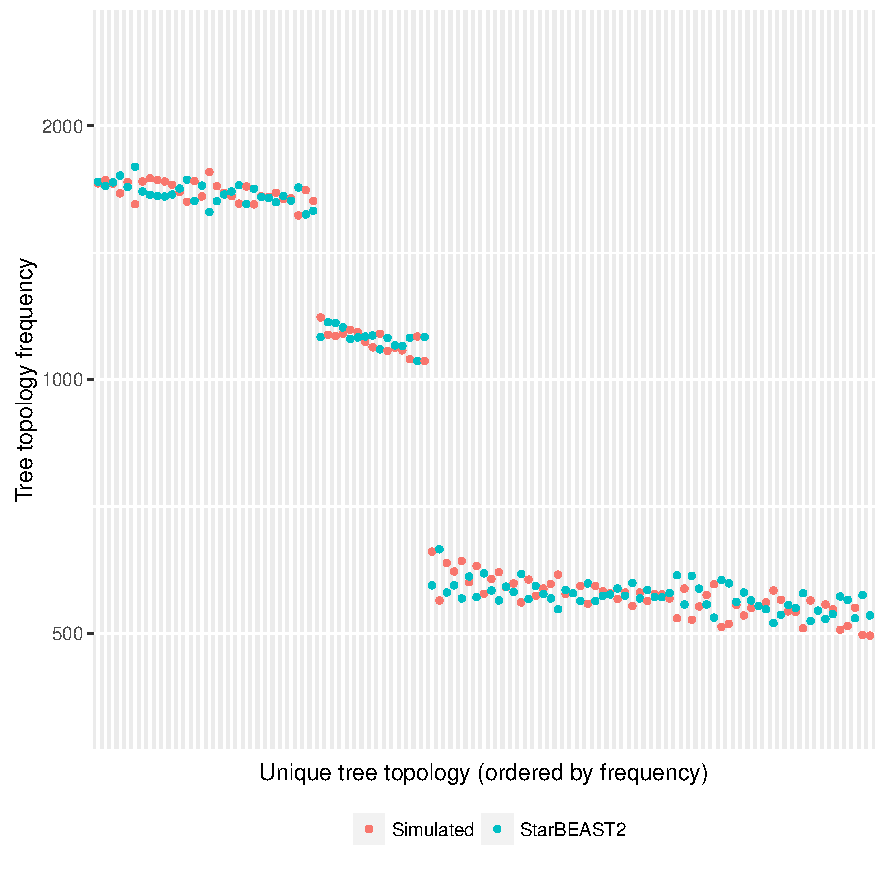
\includegraphics[width=16cm]{species_topology_frequencies.pdf}
\caption
{Frequency of five-taxon species tree topologies sampled from a birth-death prior
distribution. Topologies were sampled by simulating trees using biopy (red), or
by using a StarBEAST2 MCMC chain (blue). Frequencies are identical apart from
noise, indicating that StarBEAST2 is mathematically correct. Three levels of
probability are evident from left to right --- high probability balanced
topologies e.g. ((a,b),((c,d),e)), middle probability intermediate topologies
e.g. (((a,b),(c,d)),e), and low probability unbalanced topologies e.g.
((((a,b),c),d),e).}
\label{fig:speciesTopologyFrequencies}
\end{figure}

\clearpage

\begin{figure}[htb!]
\centering
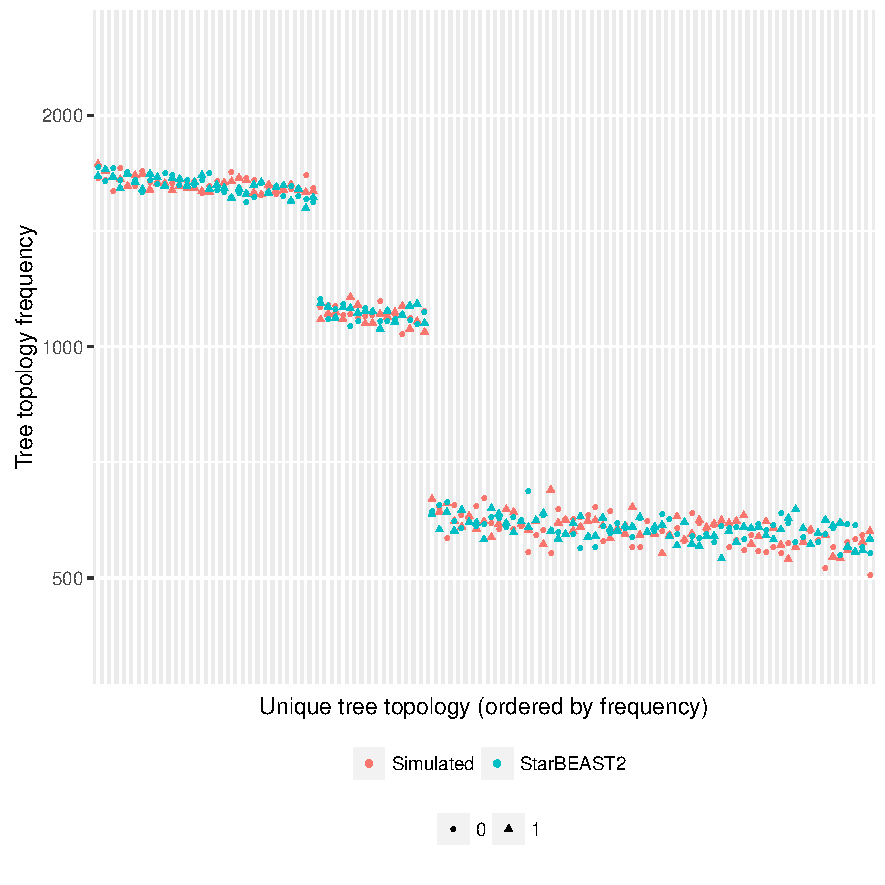
\includegraphics[width=16cm]{gene_topology_frequencies.pdf}
\caption
{Frequency of five-taxon gene tree topologies sampled from a multispecies
coalescent prior distribution. Topologies were sampled by simulating gene trees
within species trees using biopy (red), or by using a StarBEAST2 MCMC chain
(blue). Gene trees were sampled with two clock rates, 0.5 (circles) and 2.0
(triangles), although clock rate should not affect topology or node heights in
units of time. Frequencies are identical apart from noise, indicating that
StarBEAST2 is mathematically correct. Three levels of probability are evident
from left to right --- high probability balanced topologies e.g.
((a,b),((c,d),e)), middle probability intermediate topologies e.g.
(((a,b),(c,d)),e), and low probability unbalanced topologies e.g.
((((a,b),c),d),e).}
\label{fig:geneTopologyFrequencies}
\end{figure}

\clearpage

\begin{figure}[htb!]
\centering
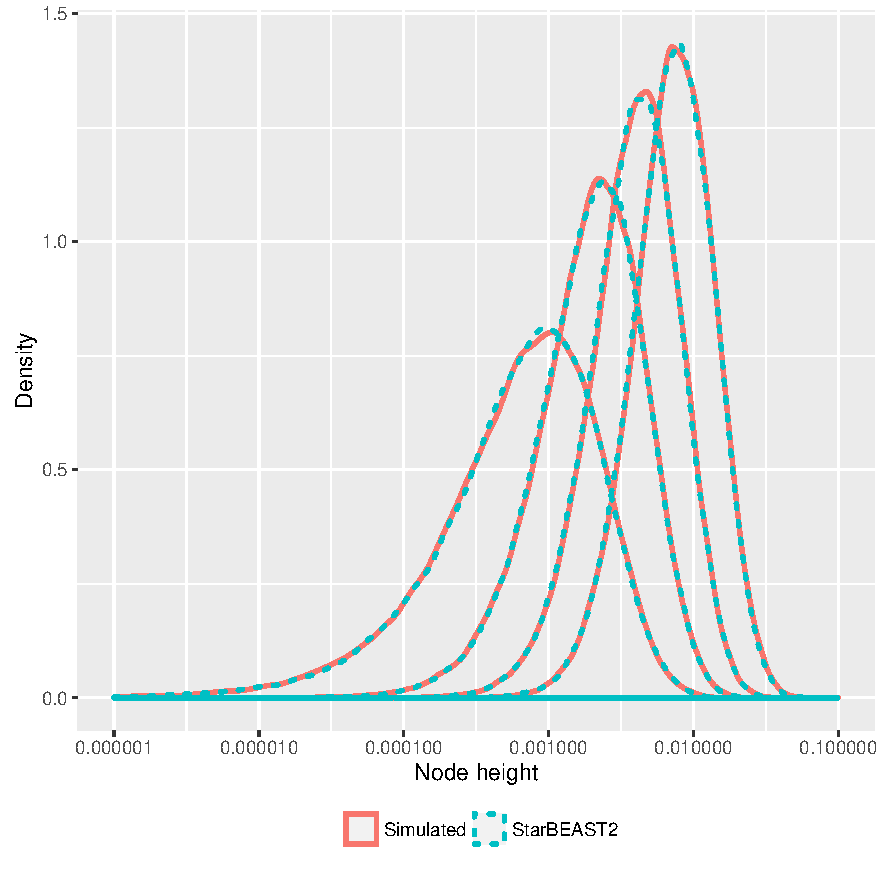
\includegraphics[width=16cm]{species_node_heights.pdf}
\caption
{Probability densities of five-taxon species tree node heights sampled from a
birth-death prior distribution. Node heights were sampled by simulating trees
using biopy (red), or by using a StarBEAST2 MCMC chain (blue). Probability
densities are plotted separately for each ranked node giving four peaks, one
for each internal node. Node height probability densities are identical apart
from noise, indicating that StarBEAST2 is mathematically correct.}
\label{fig:speciesNodeHeights}
\end{figure}

\clearpage

\begin{figure}[htb!]
\centering
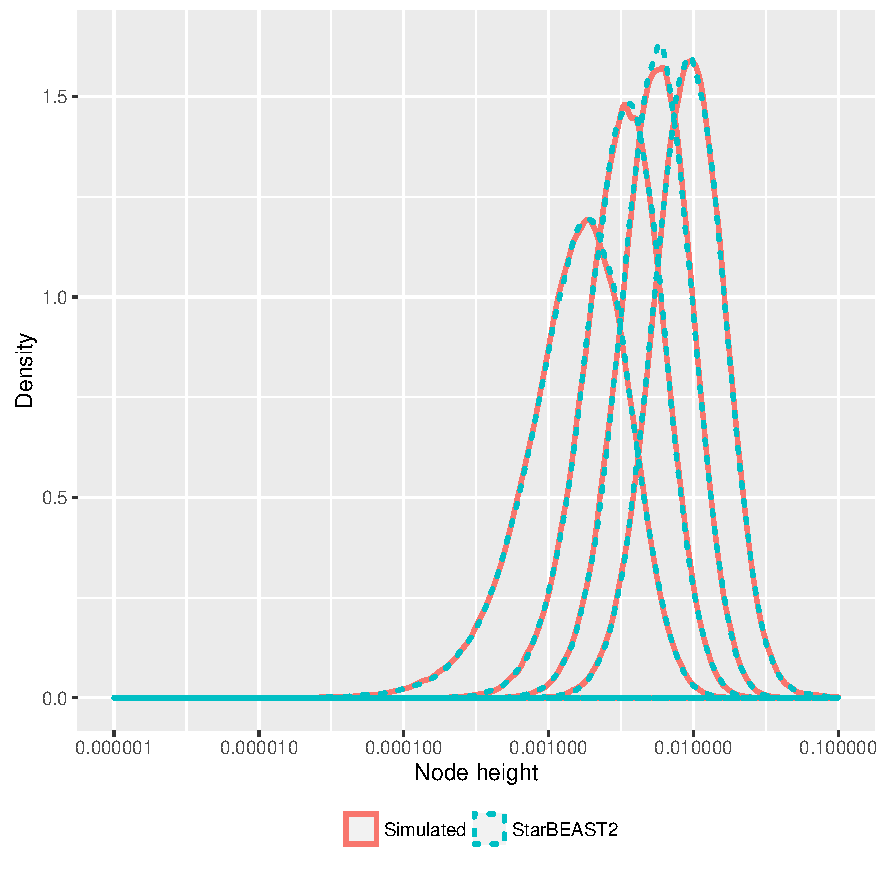
\includegraphics[width=16cm]{gene_node_heights.pdf}
\caption
{Probability densities of five-taxon gene tree node heights sampled from a
multispecies coalescent prior distribution. Node heights were sampled by
simulating gene trees within species trees using biopy (red), or by using a
StarBEAST2 MCMC chain (blue). Gene trees were sampled with two clock rates, 0.5
and 2.0, and node heights from both sets of gene trees were combined as clock
rate should not affect topology or node heights in units of time. Probability
densities are plotted separately for each ranked node giving four peaks, one for
each internal node. Node height probability densities are identical apart from
noise, indicating that StarBEAST2 is mathematically correct.}
\label{fig:geneNodeHeights}
\end{figure}

\clearpage

\begin{figure}[htb!]
\centering
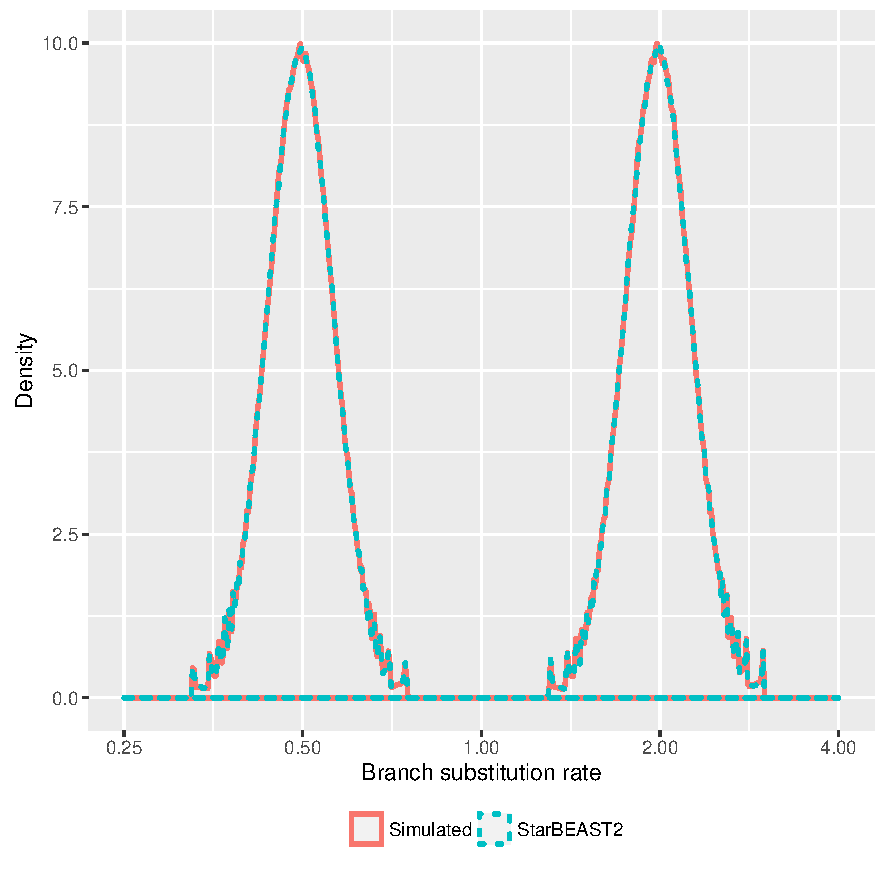
\includegraphics[width=16cm]{gene_branch_rates.pdf}
\caption
{Probability densities of five-taxon gene tree branch rates produced by a
species tree uncorrelated lognormal (UCLN) relaxed clock. Branch rates were
sampled by simulating gene trees within species trees using biopy and simulating
species tree branch rates using scipy (red), or by using a StarBEAST2 MCMC chain
(blue). Gene trees were sampled with two clock rates, 0.5 and 2.0, resulting in
two peaks. Branch rate probability densities are identical apart from noise,
indicating that StarBEAST2 is mathematically correct.}
\label{fig:geneBranchRatesUCLD}
\end{figure}

\clearpage

\begin{figure}[htb!]
\centering
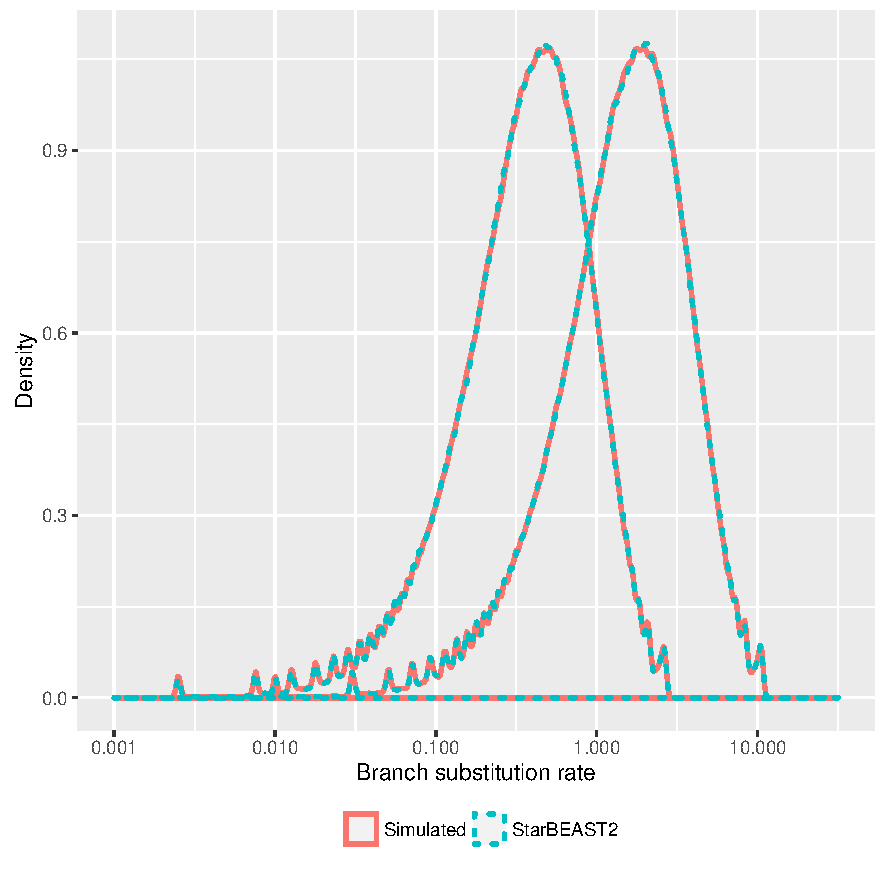
\includegraphics[width=16cm]{exp_gene_branch_rates.pdf}
\caption
{Probability densities of five-taxon gene tree branch rates produced by a
species tree uncorrelated exponential (UCED) relaxed clock. Branch rates were
sampled by simulating gene trees within species trees using biopy and simulating
species tree branch rates using scipy (red), or by using a StarBEAST2 MCMC chain
(blue). Gene trees were sampled with two clock rates, 0.5 and 2.0, resulting in
two peaks. Branch rate probability densities are identical apart from noise,
indicating that StarBEAST2 is mathematically correct.}
\label{fig:geneBranchRatesUCED}
\end{figure}

\clearpage

\begin{figure}[htb!]
\centering
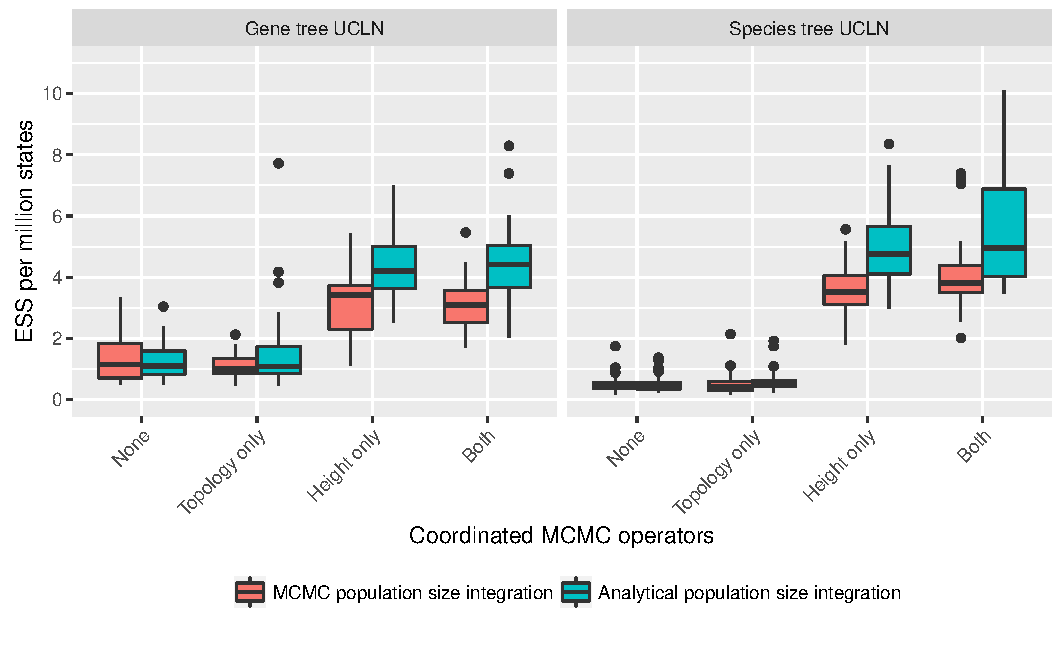
\includegraphics[width=\textwidth]{minimum_ess_per_mstates_boxplot.pdf}
\caption
{Impact of operators, population size integration and clock models on effective
sample size (ESS) per million states of \textit{Pseudacris} reanalyses. The
estimated sample size (ESS) per hour for a given replicate used the smallest ESS
out of all recorded statistics. Topology refers to the replacement of na\"ive
nearest-neighbor interchange and subtree prune and regraft operators with
coordinated operators. Height refers to the addition of operators which make
coordinated changes to node heights. Uncorrelated log-normal (UCLN) relaxed
clocks were applied to either each gene tree or to the species tree. N = 32.}
\label{fig:realEssPerMstates}
\end{figure}

\clearpage

\begin{figure}[htb!]
\centering
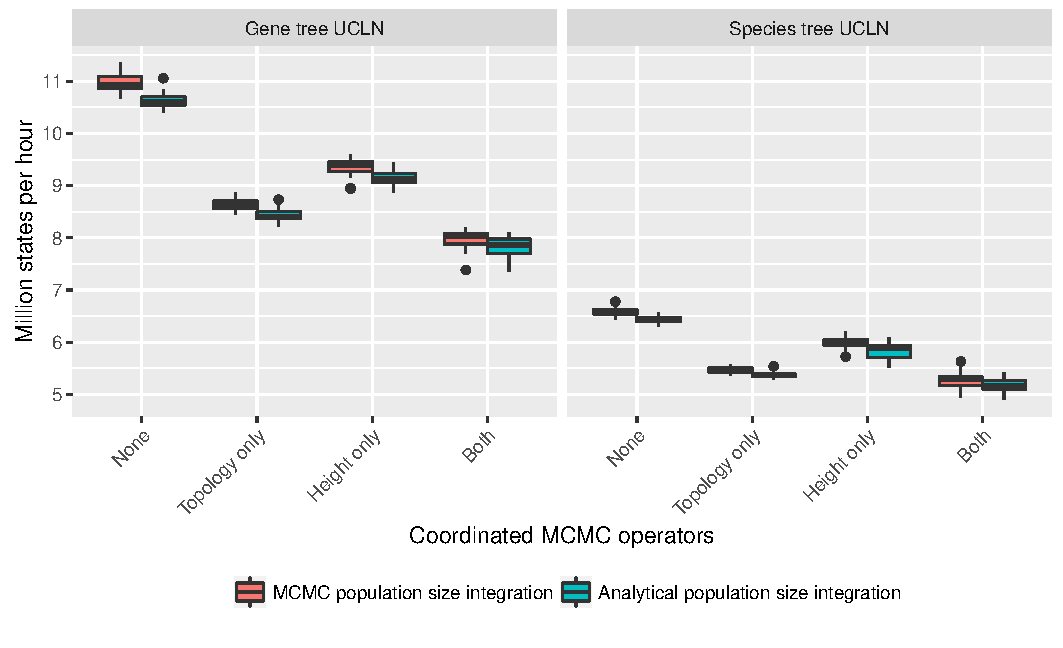
\includegraphics[width=\textwidth]{mstates_rates.pdf}
\caption
{Impact of operators, population size integration and clock models on the
calculation time for each state. The estimated sample size (ESS) per hour for a
given replicate used the smallest ESS out of all recorded statistics. Topology
refers to the replacement of na\"ive nearest-neighbor interchange and subtree
prune and regraft operators with coordinated operators. Height refers to the
addition of operators which make coordinated changes to node heights.
Uncorrelated log-normal (UCLN) relaxed clocks were applied to either each gene
tree or to the species tree. N = 32.}
\label{fig:mstatesPerHour}
\end{figure}

\clearpage

\begin{figure}[htb!]
\centering
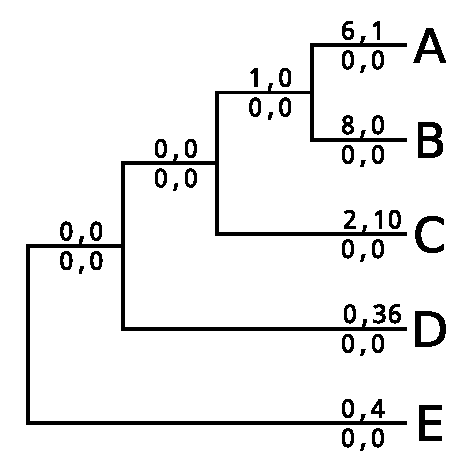
\includegraphics[width=7cm]{false_branch_rates.pdf}
\caption
{Number of erroneous per-species substitution rates estimated using BEAST concatenation and StarBEAST2. Erroneous
branch rates are those with 95\% credibility intervals which do not include the true rate of 1.
Numbers above a branch are the counts of erroneous branches for concatenation, and those
below are the counts for StarBEAST2, both out of 96 replicates. The first count is
the number of branch rates inferred to be faster than 1, and the
second is the number inferred to be slower than 1.}
\label{fig:spilsBranchRates}
\end{figure}

\begin{figure}[htb!]
\centering
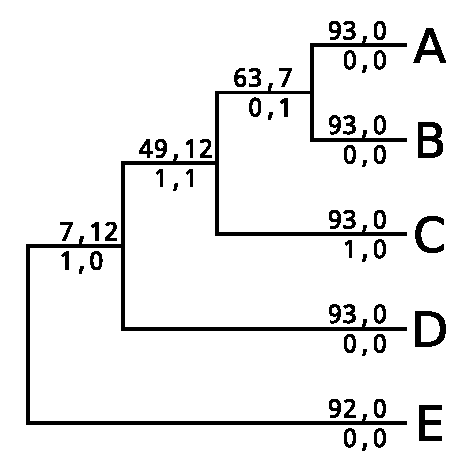
\includegraphics[width=7cm]{false_branch_lengths.pdf}
\caption
{Number of erroneous branch lengths estimated using BEAST concatenation and StarBEAST2. Erroneous
branch lengths are those with 95\% credibility intervals which do not include the true simulated length for a given branch.
Numbers above a branch are the counts of erroneous branches for concatenation, and those
below are the counts for StarBEAST2, both out of 96 replicates. The first count is
the number of branch lengths inferred to be longer than the true length, and the
second is the number inferred to be shorter.}
\label{fig:spilsBranchLengths}
\end{figure}

\clearpage

\begin{table}[htb!]
\centering
\caption{Mean log(ESS per hour) for \textit{Pseudacris} data.}
\label{tab:pseudacrisPerHour}
\begin{threeparttable}
\renewcommand{\arraystretch}{1.5}
\footnotesize
\begin{minipage}[t]{\textwidth}
\centering
$\begin{array}{|c|c|c|c|c|c|c|c|}
\multicolumn{1}{c}{} & \multicolumn{1}{c}{\ontop{\text{Birth-death}}{\text{probability}}} & \multicolumn{1}{c}{\ontop{\text{Clock rate}}{\text{stdev}}} & \multicolumn{1}{c}{\ontop{\text{Extinction}}{\text{fraction}}} & \multicolumn{1}{c}{\ontop{\text{Among-site}}{\text{rate variation}}} & \multicolumn{1}{c}{\ontop{\text{Transition/}}{\text{Transversion}} \kappa} & \multicolumn{1}{c}{\ontop{\text{Phylogenetic}}{\text{likelihood}}} & \multicolumn{1}{c}{\text{Minimum}}\tabularnewline
\hline
\lozenge\lozenge\lozenge\lozenge & \ontop{4.63}{4.51 - 4.74} & \ontop{5.36}{5.20 - 5.50} & \ontop{5.28}{5.16 - 5.40} & \ontop{5.59}{5.37 - 5.81} & \ontop{5.61}{5.40 - 5.83} & \ontop{3.28}{3.16 - 3.41} & \ontop{2.52}{2.30 - 2.72}\tabularnewline
\hline
\lozenge\lozenge\lozenge\blacklozenge & \ontop{4.86}{4.78 - 4.93} & \ontop{5.66}{5.60 - 5.72} & \ontop{5.39}{5.36 - 5.42} & \ontop{6.27}{6.17 - 6.37} & \ontop{6.35}{6.24 - 6.47} & \ontop{3.50}{3.35 - 3.62} & \ontop{3.33}{3.21 - 3.44}\tabularnewline
\hline
\lozenge\lozenge\blacklozenge\lozenge & \ontop{4.25}{4.17 - 4.32} & \ontop{5.06}{4.95 - 5.16} & \ontop{5.00}{4.91 - 5.09} & \ontop{5.25}{5.10 - 5.39} & \ontop{5.28}{5.14 - 5.43} & \ontop{2.88}{2.75 - 3.02} & \ontop{2.18}{2.05 - 2.30}\tabularnewline
\hline
\lozenge\lozenge\blacklozenge\blacklozenge & \ontop{4.65}{4.59 - 4.71} & \ontop{5.45}{5.40 - 5.51} & \ontop{5.27}{5.24 - 5.30} & \ontop{6.11}{6.02 - 6.20} & \ontop{6.21}{6.13 - 6.29} & \ontop{3.34}{3.23 - 3.45} & \ontop{3.18}{3.11 - 3.26}\tabularnewline
\hline
\lozenge\blacklozenge\lozenge\lozenge & \ontop{3.49}{3.33 - 3.65} & \ontop{4.13}{3.93 - 4.35} & \ontop{4.08}{3.87 - 4.26} & \ontop{4.16}{3.95 - 4.38} & \ontop{4.17}{3.94 - 4.39} & \ontop{2.65}{2.54 - 2.74} & \ontop{1.12}{0.98 - 1.26}\tabularnewline
\hline
\lozenge\blacklozenge\lozenge\blacklozenge & \ontop{4.49}{4.45 - 4.54} & \ontop{5.42}{5.37 - 5.48} & \ontop{5.09}{5.05 - 5.13} & \ontop{5.91}{5.81 - 6.02} & \ontop{5.98}{5.85 - 6.09} & \ontop{3.10}{3.00 - 3.20} & \ontop{3.03}{2.95 - 3.11}\tabularnewline
\hline
\lozenge\blacklozenge\blacklozenge\lozenge & \ontop{3.27}{3.11 - 3.43} & \ontop{4.00}{3.82 - 4.18} & \ontop{3.98}{3.81 - 4.16} & \ontop{4.04}{3.84 - 4.26} & \ontop{4.04}{3.83 - 4.26} & \ontop{2.53}{2.43 - 2.63} & \ontop{0.90}{0.71 - 1.11}\tabularnewline
\hline
\lozenge\blacklozenge\blacklozenge\blacklozenge & \ontop{4.42}{4.34 - 4.49} & \ontop{5.38}{5.32 - 5.45} & \ontop{4.96}{4.93 - 5.00} & \ontop{5.91}{5.81 - 6.01} & \ontop{5.98}{5.86 - 6.10} & \ontop{3.10}{3.00 - 3.20} & \ontop{3.02}{2.92 - 3.13}\tabularnewline
\hline
\blacklozenge\lozenge\lozenge\lozenge & \ontop{4.67}{4.59 - 4.74} & \ontop{5.25}{5.13 - 5.36} & \ontop{5.21}{5.12 - 5.30} & \ontop{5.44}{5.28 - 5.60} & \ontop{5.46}{5.31 - 5.62} & \ontop{3.36}{3.25 - 3.46} & \ontop{2.48}{2.33 - 2.64}\tabularnewline
\hline
\blacklozenge\lozenge\lozenge\blacklozenge & \ontop{4.96}{4.91 - 5.01} & \ontop{5.73}{5.68 - 5.78} & \ontop{5.47}{5.44 - 5.50} & \ontop{6.45}{6.36 - 6.54} & \ontop{6.59}{6.50 - 6.68} & \ontop{3.71}{3.63 - 3.81} & \ontop{3.66}{3.59 - 3.74}\tabularnewline
\hline
\blacklozenge\lozenge\blacklozenge\lozenge & \ontop{4.54}{4.44 - 4.65} & \ontop{5.20}{5.06 - 5.33} & \ontop{5.08}{5.00 - 5.17} & \ontop{5.50}{5.30 - 5.72} & \ontop{5.56}{5.35 - 5.80} & \ontop{3.12}{2.95 - 3.28} & \ontop{2.36}{2.15 - 2.58}\tabularnewline
\hline
\blacklozenge\lozenge\blacklozenge\blacklozenge & \ontop{4.79}{4.74 - 4.83} & \ontop{5.59}{5.54 - 5.64} & \ontop{5.28}{5.25 - 5.31} & \ontop{6.27}{6.18 - 6.35} & \ontop{6.40}{6.31 - 6.49} & \ontop{3.55}{3.45 - 3.66} & \ontop{3.53}{3.43 - 3.62}\tabularnewline
\hline
\blacklozenge\blacklozenge\lozenge\lozenge & \ontop{3.76}{3.62 - 3.90} & \ontop{4.25}{4.09 - 4.42} & \ontop{4.23}{4.05 - 4.38} & \ontop{4.31}{4.12 - 4.48} & \ontop{4.30}{4.13 - 4.48} & \ontop{2.83}{2.77 - 2.89} & \ontop{1.16}{1.01 - 1.31}\tabularnewline
\hline
\blacklozenge\blacklozenge\lozenge\blacklozenge & \ontop{4.60}{4.54 - 4.66} & \ontop{5.56}{5.50 - 5.62} & \ontop{5.11}{5.07 - 5.15} & \ontop{6.15}{6.07 - 6.23} & \ontop{6.27}{6.17 - 6.36} & \ontop{3.39}{3.28 - 3.48} & \ontop{3.36}{3.28 - 3.46}\tabularnewline
\hline
\blacklozenge\blacklozenge\blacklozenge\lozenge & \ontop{3.57}{3.42 - 3.72} & \ontop{4.14}{3.97 - 4.32} & \ontop{4.10}{3.93 - 4.26} & \ontop{4.18}{3.97 - 4.38} & \ontop{4.19}{3.99 - 4.40} & \ontop{2.71}{2.63 - 2.79} & \ontop{1.05}{0.91 - 1.22}\tabularnewline
\hline
\blacklozenge\blacklozenge\blacklozenge\blacklozenge & \ontop{4.45}{4.36 - 4.52} & \ontop{5.47}{5.39 - 5.53} & \ontop{4.99}{4.95 - 5.02} & \ontop{6.17}{6.11 - 6.24} & \ontop{6.26}{6.20 - 6.32} & \ontop{3.32}{3.21 - 3.44} & \ontop{3.31}{3.21 - 3.42}\tabularnewline
\hline
\multicolumn{1}{c}{} & \multicolumn{1}{c}{\ontop{\text{Diversification}}{\text{rate}}} & \multicolumn{1}{c}{\ontop{\text{Population}}{\text{Mean}}} & \multicolumn{1}{c}{\text{Log-posterior}} & \multicolumn{1}{c}{\text{Log-prior}} & \multicolumn{1}{c}{\ontop{\text{Species}}{\text{tree height}}} & \multicolumn{1}{c}{\ontop{\text{Species}}{\text{tree length}}} & \multicolumn{1}{c}{\ontop{\text{Coalescent}}{\text{probability}}}\tabularnewline
\hline
\lozenge\lozenge\lozenge\lozenge & \ontop{5.31}{5.18 - 5.45} & \ontop{3.51}{3.40 - 3.61} & \ontop{3.36}{3.25 - 3.50} & \ontop{3.61}{3.53 - 3.70} & \ontop{2.54}{2.34 - 2.72} & \ontop{4.39}{4.26 - 4.52} & \ontop{3.19}{3.08 - 3.31}\tabularnewline
\hline
\lozenge\lozenge\lozenge\blacklozenge & \ontop{5.45}{5.41 - 5.48} & \ontop{3.79}{3.69 - 3.88} & \ontop{3.75}{3.67 - 3.83} & \ontop{3.75}{3.67 - 3.83} & \ontop{4.50}{4.44 - 4.56} & \ontop{4.66}{4.58 - 4.73} & \ontop{3.51}{3.42 - 3.60}\tabularnewline
\hline
\lozenge\lozenge\blacklozenge\lozenge & \ontop{5.03}{4.93 - 5.13} & \ontop{3.23}{3.17 - 3.30} & \ontop{3.13}{3.04 - 3.21} & \ontop{3.29}{3.20 - 3.38} & \ontop{2.20}{2.07 - 2.32} & \ontop{4.07}{3.99 - 4.15} & \ontop{2.95}{2.85 - 3.04}\tabularnewline
\hline
\lozenge\lozenge\blacklozenge\blacklozenge & \ontop{5.31}{5.28 - 5.34} & \ontop{3.63}{3.54 - 3.71} & \ontop{3.58}{3.50 - 3.66} & \ontop{3.52}{3.44 - 3.61} & \ontop{4.34}{4.28 - 4.40} & \ontop{4.49}{4.42 - 4.55} & \ontop{3.33}{3.24 - 3.42}\tabularnewline
\hline
\lozenge\blacklozenge\lozenge\lozenge & \ontop{4.10}{3.92 - 4.28} & \ontop{3.04}{2.95 - 3.14} & \ontop{2.99}{2.88 - 3.09} & \ontop{2.89}{2.77 - 2.99} & \ontop{1.12}{0.97 - 1.28} & \ontop{3.03}{2.85 - 3.21} & \ontop{2.83}{2.73 - 2.92}\tabularnewline
\hline
\lozenge\blacklozenge\lozenge\blacklozenge & \ontop{5.10}{5.04 - 5.14} & \ontop{3.44}{3.35 - 3.53} & \ontop{3.46}{3.37 - 3.55} & \ontop{3.37}{3.30 - 3.44} & \ontop{3.87}{3.81 - 3.93} & \ontop{4.27}{4.22 - 4.33} & \ontop{3.22}{3.12 - 3.31}\tabularnewline
\hline
\lozenge\blacklozenge\blacklozenge\lozenge & \ontop{3.94}{3.76 - 4.13} & \ontop{2.84}{2.76 - 2.93} & \ontop{2.79}{2.69 - 2.91} & \ontop{2.78}{2.69 - 2.88} & \ontop{0.90}{0.71 - 1.10} & \ontop{2.78}{2.55 - 3.00} & \ontop{2.67}{2.58 - 2.75}\tabularnewline
\hline
\lozenge\blacklozenge\blacklozenge\blacklozenge & \ontop{5.02}{4.97 - 5.06} & \ontop{3.43}{3.33 - 3.52} & \ontop{3.44}{3.36 - 3.51} & \ontop{3.32}{3.25 - 3.40} & \ontop{3.88}{3.82 - 3.94} & \ontop{4.20}{4.12 - 4.28} & \ontop{3.20}{3.11 - 3.30}\tabularnewline
\hline
\blacklozenge\lozenge\lozenge\lozenge & \ontop{5.22}{5.11 - 5.31} & \ontop{3.98}{3.90 - 4.06} & \ontop{3.69}{3.58 - 3.80} & \ontop{5.05}{4.94 - 5.15} & \ontop{2.48}{2.34 - 2.64} & \ontop{4.46}{4.36 - 4.56} & \ontop{3.56}{3.46 - 3.65}\tabularnewline
\hline
\blacklozenge\lozenge\lozenge\blacklozenge & \ontop{5.52}{5.48 - 5.56} & \ontop{4.39}{4.31 - 4.47} & \ontop{4.15}{4.07 - 4.22} & \ontop{5.46}{5.40 - 5.51} & \ontop{4.68}{4.63 - 4.72} & \ontop{4.75}{4.70 - 4.81} & \ontop{3.88}{3.81 - 3.96}\tabularnewline
\hline
\blacklozenge\lozenge\blacklozenge\lozenge & \ontop{5.12}{5.02 - 5.21} & \ontop{3.83}{3.71 - 3.95} & \ontop{3.51}{3.35 - 3.67} & \ontop{4.98}{4.86 - 5.09} & \ontop{2.40}{2.17 - 2.66} & \ontop{4.32}{4.19 - 4.44} & \ontop{3.42}{3.29 - 3.55}\tabularnewline
\hline
\blacklozenge\lozenge\blacklozenge\blacklozenge & \ontop{5.30}{5.27 - 5.33} & \ontop{4.32}{4.25 - 4.39} & \ontop{4.03}{3.95 - 4.09} & \ontop{5.33}{5.28 - 5.38} & \ontop{4.57}{4.53 - 4.61} & \ontop{4.60}{4.55 - 4.64} & \ontop{3.80}{3.72 - 3.88}\tabularnewline
\hline
\blacklozenge\blacklozenge\lozenge\lozenge & \ontop{4.19}{4.04 - 4.35} & \ontop{3.56}{3.48 - 3.64} & \ontop{3.33}{3.25 - 3.42} & \ontop{4.10}{3.96 - 4.24} & \ontop{1.16}{1.00 - 1.33} & \ontop{3.42}{3.26 - 3.60} & \ontop{3.24}{3.16 - 3.32}\tabularnewline
\hline
\blacklozenge\blacklozenge\lozenge\blacklozenge & \ontop{5.16}{5.13 - 5.20} & \ontop{4.23}{4.17 - 4.29} & \ontop{3.93}{3.87 - 3.99} & \ontop{5.31}{5.25 - 5.37} & \ontop{4.11}{4.05 - 4.18} & \ontop{4.43}{4.38 - 4.48} & \ontop{3.71}{3.64 - 3.78}\tabularnewline
\hline
\blacklozenge\blacklozenge\blacklozenge\lozenge & \ontop{4.08}{3.92 - 4.25} & \ontop{3.35}{3.25 - 3.45} & \ontop{3.18}{3.09 - 3.27} & \ontop{3.93}{3.75 - 4.11} & \ontop{1.05}{0.89 - 1.22} & \ontop{3.01}{2.81 - 3.22} & \ontop{3.09}{3.01 - 3.16}\tabularnewline
\hline
\blacklozenge\blacklozenge\blacklozenge\blacklozenge & \ontop{5.03}{5.00 - 5.07} & \ontop{4.19}{4.11 - 4.28} & \ontop{3.89}{3.81 - 3.96} & \ontop{5.26}{5.20 - 5.32} & \ontop{3.96}{3.88 - 4.06} & \ontop{4.27}{4.19 - 4.35} & \ontop{3.68}{3.61 - 3.76}\tabularnewline
\hline
\end{array}$
\end{minipage}
\begin{tablenotes}
\scriptsize
\item Bottom numbers show 95\% confidence intervals for the mean calculated by bootstrapping
\item Filled diamonds indicate which new features are enabled. From left-to-right; analytical integration of population sizes, species tree relaxed clocks, coordinated topology operators, and coordinated height operators.
\end{tablenotes}
\end{threeparttable}
\end{table}

\clearpage

\begin{table}[htb!]
\centering
\caption{Mean log(ESS per million states) for \textit{Pseudacris} data.}
\label{tab:pseudacrisPerMstates}
\begin{threeparttable}
\renewcommand{\arraystretch}{1.5}
\footnotesize
\begin{minipage}[t]{\textwidth}
\centering
$\begin{array}{|c|c|c|c|c|c|c|c|}
\multicolumn{1}{c}{} & \multicolumn{1}{c}{\ontop{\text{Birth-death}}{\text{probability}}} & \multicolumn{1}{c}{\ontop{\text{Clock rate}}{\text{stdev}}} & \multicolumn{1}{c}{\ontop{\text{Extinction}}{\text{fraction}}} & \multicolumn{1}{c}{\ontop{\text{Among-site}}{\text{rate variation}}} & \multicolumn{1}{c}{\ontop{\text{Transition/}}{\text{Transversion}} \kappa} & \multicolumn{1}{c}{\ontop{\text{Phylogenetic}}{\text{likelihood}}} & \multicolumn{1}{c}{\text{Minimum}}\tabularnewline
\hline
\lozenge\lozenge\lozenge\lozenge & \ontop{2.23}{2.12 - 2.34} & \ontop{2.96}{2.81 - 3.10} & \ontop{2.88}{2.76 - 3.00} & \ontop{3.19}{2.99 - 3.40} & \ontop{3.22}{3.00 - 3.43} & \ontop{0.88}{0.75 - 1.02} & \ontop{0.13}{-0.06 - 0.33}\tabularnewline
\hline
\lozenge\lozenge\lozenge\blacklozenge & \ontop{2.62}{2.56 - 2.69} & \ontop{3.42}{3.37 - 3.48} & \ontop{3.16}{3.13 - 3.19} & \ontop{4.03}{3.93 - 4.12} & \ontop{4.11}{3.99 - 4.22} & \ontop{1.26}{1.13 - 1.38} & \ontop{1.09}{0.98 - 1.21}\tabularnewline
\hline
\lozenge\lozenge\blacklozenge\lozenge & \ontop{2.09}{2.02 - 2.16} & \ontop{2.90}{2.79 - 3.00} & \ontop{2.85}{2.75 - 2.93} & \ontop{3.09}{2.95 - 3.25} & \ontop{3.13}{2.97 - 3.28} & \ontop{0.73}{0.59 - 0.85} & \ontop{0.02}{-0.09 - 0.14}\tabularnewline
\hline
\lozenge\lozenge\blacklozenge\blacklozenge & \ontop{2.57}{2.51 - 2.63} & \ontop{3.38}{3.32 - 3.43} & \ontop{3.19}{3.17 - 3.23} & \ontop{4.03}{3.94 - 4.12} & \ontop{4.13}{4.06 - 4.21} & \ontop{1.26}{1.16 - 1.36} & \ontop{1.11}{1.03 - 1.19}\tabularnewline
\hline
\lozenge\blacklozenge\lozenge\lozenge & \ontop{1.61}{1.45 - 1.76} & \ontop{2.25}{2.05 - 2.46} & \ontop{2.19}{2.01 - 2.38} & \ontop{2.27}{2.05 - 2.48} & \ontop{2.29}{2.04 - 2.53} & \ontop{0.77}{0.67 - 0.85} & \ontop{-0.77}{-0.91 - -0.62}\tabularnewline
\hline
\lozenge\blacklozenge\lozenge\blacklozenge & \ontop{2.70}{2.66 - 2.74} & \ontop{3.63}{3.58 - 3.69} & \ontop{3.30}{3.26 - 3.33} & \ontop{4.12}{4.02 - 4.22} & \ontop{4.18}{4.07 - 4.29} & \ontop{1.31}{1.21 - 1.41} & \ontop{1.24}{1.15 - 1.32}\tabularnewline
\hline
\lozenge\blacklozenge\blacklozenge\lozenge & \ontop{1.57}{1.41 - 1.74} & \ontop{2.30}{2.13 - 2.49} & \ontop{2.28}{2.10 - 2.45} & \ontop{2.34}{2.13 - 2.57} & \ontop{2.34}{2.14 - 2.54} & \ontop{0.83}{0.73 - 0.93} & \ontop{-0.80}{-1.00 - -0.60}\tabularnewline
\hline
\lozenge\blacklozenge\blacklozenge\blacklozenge & \ontop{2.76}{2.69 - 2.82} & \ontop{3.72}{3.66 - 3.79} & \ontop{3.31}{3.27 - 3.34} & \ontop{4.25}{4.15 - 4.35} & \ontop{4.32}{4.20 - 4.43} & \ontop{1.44}{1.34 - 1.54} & \ontop{1.36}{1.27 - 1.46}\tabularnewline
\hline
\blacklozenge\lozenge\lozenge\lozenge & \ontop{2.30}{2.23 - 2.38} & \ontop{2.88}{2.76 - 2.99} & \ontop{2.84}{2.74 - 2.94} & \ontop{3.08}{2.92 - 3.24} & \ontop{3.10}{2.95 - 3.25} & \ontop{0.99}{0.89 - 1.09} & \ontop{0.12}{-0.04 - 0.27}\tabularnewline
\hline
\blacklozenge\lozenge\lozenge\blacklozenge & \ontop{2.75}{2.70 - 2.79} & \ontop{3.51}{3.46 - 3.57} & \ontop{3.25}{3.23 - 3.28} & \ontop{4.24}{4.15 - 4.32} & \ontop{4.38}{4.29 - 4.46} & \ontop{1.50}{1.41 - 1.59} & \ontop{1.45}{1.37 - 1.53}\tabularnewline
\hline
\blacklozenge\lozenge\blacklozenge\lozenge & \ontop{2.41}{2.30 - 2.51} & \ontop{3.07}{2.95 - 3.19} & \ontop{2.95}{2.87 - 3.04} & \ontop{3.37}{3.17 - 3.56} & \ontop{3.43}{3.22 - 3.66} & \ontop{0.99}{0.84 - 1.15} & \ontop{0.23}{0.03 - 0.46}\tabularnewline
\hline
\blacklozenge\lozenge\blacklozenge\blacklozenge & \ontop{2.73}{2.68 - 2.77} & \ontop{3.53}{3.47 - 3.59} & \ontop{3.22}{3.19 - 3.25} & \ontop{4.21}{4.12 - 4.30} & \ontop{4.35}{4.26 - 4.43} & \ontop{1.49}{1.39 - 1.60} & \ontop{1.47}{1.38 - 1.56}\tabularnewline
\hline
\blacklozenge\blacklozenge\lozenge\lozenge & \ontop{1.90}{1.75 - 2.05} & \ontop{2.39}{2.22 - 2.55} & \ontop{2.36}{2.19 - 2.54} & \ontop{2.44}{2.26 - 2.60} & \ontop{2.43}{2.26 - 2.61} & \ontop{0.97}{0.91 - 1.03} & \ontop{-0.70}{-0.85 - -0.55}\tabularnewline
\hline
\blacklozenge\blacklozenge\lozenge\blacklozenge & \ontop{2.84}{2.78 - 2.90} & \ontop{3.79}{3.73 - 3.86} & \ontop{3.35}{3.30 - 3.38} & \ontop{4.39}{4.30 - 4.46} & \ontop{4.50}{4.41 - 4.59} & \ontop{1.62}{1.52 - 1.73} & \ontop{1.60}{1.51 - 1.69}\tabularnewline
\hline
\blacklozenge\blacklozenge\blacklozenge\lozenge & \ontop{1.89}{1.74 - 2.02} & \ontop{2.46}{2.29 - 2.64} & \ontop{2.42}{2.25 - 2.58} & \ontop{2.50}{2.31 - 2.70} & \ontop{2.51}{2.29 - 2.73} & \ontop{1.03}{0.96 - 1.11} & \ontop{-0.63}{-0.77 - -0.47}\tabularnewline
\hline
\blacklozenge\blacklozenge\blacklozenge\blacklozenge & \ontop{2.81}{2.72 - 2.88} & \ontop{3.82}{3.74 - 3.90} & \ontop{3.34}{3.30 - 3.38} & \ontop{4.53}{4.46 - 4.59} & \ontop{4.61}{4.55 - 4.67} & \ontop{1.67}{1.57 - 1.78} & \ontop{1.66}{1.56 - 1.78}\tabularnewline
\hline
\multicolumn{1}{c}{} & \multicolumn{1}{c}{\ontop{\text{Diversification}}{\text{rate}}} & \multicolumn{1}{c}{\ontop{\text{Population}}{\text{Mean}}} & \multicolumn{1}{c}{\text{Log-posterior}} & \multicolumn{1}{c}{\text{Log-prior}} & \multicolumn{1}{c}{\ontop{\text{Species}}{\text{tree height}}} & \multicolumn{1}{c}{\ontop{\text{Species}}{\text{tree length}}} & \multicolumn{1}{c}{\ontop{\text{Coalescent}}{\text{probability}}}\tabularnewline
\hline
\lozenge\lozenge\lozenge\lozenge & \ontop{2.91}{2.77 - 3.03} & \ontop{1.11}{1.01 - 1.20} & \ontop{0.97}{0.85 - 1.09} & \ontop{1.22}{1.14 - 1.29} & \ontop{0.14}{-0.05 - 0.32} & \ontop{2.00}{1.87 - 2.12} & \ontop{0.80}{0.68 - 0.92}\tabularnewline
\hline
\lozenge\lozenge\lozenge\blacklozenge & \ontop{3.21}{3.18 - 3.24} & \ontop{1.56}{1.46 - 1.65} & \ontop{1.51}{1.44 - 1.59} & \ontop{1.51}{1.44 - 1.59} & \ontop{2.27}{2.20 - 2.33} & \ontop{2.42}{2.35 - 2.48} & \ontop{1.28}{1.18 - 1.37}\tabularnewline
\hline
\lozenge\lozenge\blacklozenge\lozenge & \ontop{2.88}{2.77 - 2.97} & \ontop{1.08}{1.02 - 1.13} & \ontop{0.97}{0.89 - 1.05} & \ontop{1.14}{1.04 - 1.22} & \ontop{0.04}{-0.09 - 0.16} & \ontop{1.91}{1.84 - 1.99} & \ontop{0.79}{0.70 - 0.88}\tabularnewline
\hline
\lozenge\lozenge\blacklozenge\blacklozenge & \ontop{3.23}{3.20 - 3.27} & \ontop{1.55}{1.46 - 1.63} & \ontop{1.50}{1.42 - 1.59} & \ontop{1.45}{1.37 - 1.53} & \ontop{2.26}{2.20 - 2.32} & \ontop{2.41}{2.35 - 2.47} & \ontop{1.25}{1.16 - 1.34}\tabularnewline
\hline
\lozenge\blacklozenge\lozenge\lozenge & \ontop{2.21}{2.01 - 2.39} & \ontop{1.15}{1.05 - 1.25} & \ontop{1.10}{1.00 - 1.22} & \ontop{1.01}{0.90 - 1.11} & \ontop{-0.77}{-0.92 - -0.60} & \ontop{1.15}{0.98 - 1.34} & \ontop{0.95}{0.85 - 1.03}\tabularnewline
\hline
\lozenge\blacklozenge\lozenge\blacklozenge & \ontop{3.31}{3.26 - 3.35} & \ontop{1.65}{1.56 - 1.73} & \ontop{1.67}{1.58 - 1.76} & \ontop{1.58}{1.51 - 1.65} & \ontop{2.08}{2.01 - 2.15} & \ontop{2.48}{2.43 - 2.53} & \ontop{1.43}{1.34 - 1.52}\tabularnewline
\hline
\lozenge\blacklozenge\blacklozenge\lozenge & \ontop{2.24}{2.07 - 2.41} & \ontop{1.14}{1.05 - 1.23} & \ontop{1.09}{1.00 - 1.21} & \ontop{1.08}{0.99 - 1.18} & \ontop{-0.80}{-1.01 - -0.60} & \ontop{1.08}{0.83 - 1.32} & \ontop{0.97}{0.89 - 1.04}\tabularnewline
\hline
\lozenge\blacklozenge\blacklozenge\blacklozenge & \ontop{3.36}{3.32 - 3.40} & \ontop{1.77}{1.67 - 1.85} & \ontop{1.78}{1.71 - 1.84} & \ontop{1.66}{1.59 - 1.73} & \ontop{2.22}{2.16 - 2.27} & \ontop{2.54}{2.47 - 2.61} & \ontop{1.54}{1.45 - 1.63}\tabularnewline
\hline
\blacklozenge\lozenge\lozenge\lozenge & \ontop{2.85}{2.75 - 2.95} & \ontop{1.62}{1.54 - 1.70} & \ontop{1.33}{1.22 - 1.43} & \ontop{2.69}{2.59 - 2.79} & \ontop{0.12}{-0.03 - 0.28} & \ontop{2.10}{2.00 - 2.20} & \ontop{1.20}{1.11 - 1.28}\tabularnewline
\hline
\blacklozenge\lozenge\lozenge\blacklozenge & \ontop{3.31}{3.26 - 3.35} & \ontop{2.18}{2.10 - 2.25} & \ontop{1.94}{1.86 - 2.01} & \ontop{3.24}{3.19 - 3.30} & \ontop{2.46}{2.42 - 2.51} & \ontop{2.54}{2.49 - 2.59} & \ontop{1.67}{1.59 - 1.75}\tabularnewline
\hline
\blacklozenge\lozenge\blacklozenge\lozenge & \ontop{2.99}{2.88 - 3.09} & \ontop{1.70}{1.58 - 1.81} & \ontop{1.38}{1.20 - 1.54} & \ontop{2.85}{2.74 - 2.95} & \ontop{0.27}{0.04 - 0.52} & \ontop{2.19}{2.07 - 2.30} & \ontop{1.28}{1.15 - 1.42}\tabularnewline
\hline
\blacklozenge\lozenge\blacklozenge\blacklozenge & \ontop{3.24}{3.21 - 3.28} & \ontop{2.26}{2.19 - 2.33} & \ontop{1.97}{1.90 - 2.04} & \ontop{3.27}{3.22 - 3.32} & \ontop{2.51}{2.47 - 2.54} & \ontop{2.54}{2.50 - 2.58} & \ontop{1.74}{1.67 - 1.82}\tabularnewline
\hline
\blacklozenge\blacklozenge\lozenge\lozenge & \ontop{2.33}{2.17 - 2.47} & \ontop{1.70}{1.62 - 1.77} & \ontop{1.47}{1.38 - 1.55} & \ontop{2.24}{2.08 - 2.37} & \ontop{-0.70}{-0.86 - -0.53} & \ontop{1.56}{1.39 - 1.72} & \ontop{1.38}{1.30 - 1.45}\tabularnewline
\hline
\blacklozenge\blacklozenge\lozenge\blacklozenge & \ontop{3.40}{3.36 - 3.44} & \ontop{2.47}{2.40 - 2.53} & \ontop{2.17}{2.11 - 2.23} & \ontop{3.55}{3.49 - 3.61} & \ontop{2.35}{2.28 - 2.41} & \ontop{2.66}{2.61 - 2.71} & \ontop{1.95}{1.88 - 2.01}\tabularnewline
\hline
\blacklozenge\blacklozenge\blacklozenge\lozenge & \ontop{2.40}{2.22 - 2.57} & \ontop{1.67}{1.57 - 1.78} & \ontop{1.50}{1.41 - 1.59} & \ontop{2.25}{2.07 - 2.41} & \ontop{-0.63}{-0.78 - -0.46} & \ontop{1.33}{1.11 - 1.55} & \ontop{1.41}{1.33 - 1.48}\tabularnewline
\hline
\blacklozenge\blacklozenge\blacklozenge\blacklozenge & \ontop{3.39}{3.35 - 3.42} & \ontop{2.55}{2.47 - 2.63} & \ontop{2.25}{2.17 - 2.32} & \ontop{3.61}{3.55 - 3.67} & \ontop{2.32}{2.22 - 2.41} & \ontop{2.63}{2.55 - 2.71} & \ontop{2.04}{1.96 - 2.12}\tabularnewline
\hline
\end{array}$
\end{minipage}
\begin{tablenotes}
\scriptsize
\item Bottom numbers show 95\% confidence intervals for the mean calculated by bootstrapping
\item Filled diamonds indicate which new features are enabled. From left-to-right; analytical integration of population sizes, species tree relaxed clocks, coordinated topology operators, and coordinated height operators.
\end{tablenotes}
\end{threeparttable}
\end{table}

\clearpage

\begin{table}[htb!]
\centering
\caption{Standard deviation of log(ESS per hour) for \textit{Pseudacris} data.}
\label{tab:pseudacrisPerHourSD}
\begin{threeparttable}
\renewcommand{\arraystretch}{1.5}
\footnotesize
\begin{minipage}[t]{\textwidth}
\centering
$\begin{array}{|c|c|c|c|c|c|c|c|}
\multicolumn{1}{c}{} & \multicolumn{1}{c}{\ontop{\text{Birth-death}}{\text{probability}}} & \multicolumn{1}{c}{\ontop{\text{Clock rate}}{\text{stdev}}} & \multicolumn{1}{c}{\ontop{\text{Extinction}}{\text{fraction}}} & \multicolumn{1}{c}{\ontop{\text{Among-site}}{\text{rate variation}}} & \multicolumn{1}{c}{\ontop{\text{Transition/}}{\text{Transversion}} \kappa} & \multicolumn{1}{c}{\ontop{\text{Phylogenetic}}{\text{likelihood}}} & \multicolumn{1}{c}{\text{Minimum}}\tabularnewline
\hline
\lozenge\lozenge\lozenge\lozenge & \ontop{0.33}{0.25 - 0.39} & \ontop{0.44}{0.34 - 0.51} & \ontop{0.37}{0.26 - 0.45} & \ontop{0.63}{0.53 - 0.72} & \ontop{0.64}{0.53 - 0.73} & \ontop{0.38}{0.26 - 0.47} & \ontop{0.55}{0.45 - 0.63}\tabularnewline
\hline
\lozenge\lozenge\lozenge\blacklozenge & \ontop{0.20}{0.13 - 0.25} & \ontop{0.16}{0.11 - 0.19} & \ontop{0.09}{0.07 - 0.10} & \ontop{0.29}{0.22 - 0.35} & \ontop{0.34}{0.26 - 0.41} & \ontop{0.39}{0.27 - 0.49} & \ontop{0.34}{0.25 - 0.42}\tabularnewline
\hline
\lozenge\lozenge\blacklozenge\lozenge & \ontop{0.22}{0.16 - 0.26} & \ontop{0.31}{0.24 - 0.38} & \ontop{0.28}{0.19 - 0.35} & \ontop{0.44}{0.32 - 0.55} & \ontop{0.45}{0.33 - 0.57} & \ontop{0.40}{0.30 - 0.48} & \ontop{0.36}{0.26 - 0.44}\tabularnewline
\hline
\lozenge\lozenge\blacklozenge\blacklozenge & \ontop{0.17}{0.14 - 0.20} & \ontop{0.16}{0.12 - 0.20} & \ontop{0.08}{0.06 - 0.10} & \ontop{0.27}{0.20 - 0.31} & \ontop{0.24}{0.17 - 0.27} & \ontop{0.31}{0.24 - 0.38} & \ontop{0.23}{0.17 - 0.29}\tabularnewline
\hline
\lozenge\blacklozenge\lozenge\lozenge & \ontop{0.46}{0.33 - 0.56} & \ontop{0.63}{0.44 - 0.79} & \ontop{0.56}{0.40 - 0.71} & \ontop{0.64}{0.45 - 0.81} & \ontop{0.67}{0.44 - 0.85} & \ontop{0.28}{0.16 - 0.40} & \ontop{0.44}{0.29 - 0.56}\tabularnewline
\hline
\lozenge\blacklozenge\lozenge\blacklozenge & \ontop{0.13}{0.10 - 0.15} & \ontop{0.16}{0.12 - 0.20} & \ontop{0.11}{0.08 - 0.13} & \ontop{0.30}{0.22 - 0.37} & \ontop{0.34}{0.27 - 0.42} & \ontop{0.29}{0.21 - 0.35} & \ontop{0.24}{0.17 - 0.29}\tabularnewline
\hline
\lozenge\blacklozenge\blacklozenge\lozenge & \ontop{0.47}{0.35 - 0.57} & \ontop{0.53}{0.40 - 0.63} & \ontop{0.51}{0.38 - 0.61} & \ontop{0.62}{0.42 - 0.75} & \ontop{0.60}{0.41 - 0.72} & \ontop{0.29}{0.20 - 0.37} & \ontop{0.58}{0.42 - 0.70}\tabularnewline
\hline
\lozenge\blacklozenge\blacklozenge\blacklozenge & \ontop{0.21}{0.15 - 0.27} & \ontop{0.19}{0.15 - 0.23} & \ontop{0.11}{0.08 - 0.13} & \ontop{0.30}{0.24 - 0.35} & \ontop{0.35}{0.29 - 0.40} & \ontop{0.31}{0.22 - 0.37} & \ontop{0.29}{0.19 - 0.37}\tabularnewline
\hline
\blacklozenge\lozenge\lozenge\lozenge & \ontop{0.22}{0.16 - 0.28} & \ontop{0.34}{0.24 - 0.43} & \ontop{0.28}{0.21 - 0.35} & \ontop{0.47}{0.35 - 0.58} & \ontop{0.45}{0.34 - 0.55} & \ontop{0.28}{0.22 - 0.34} & \ontop{0.44}{0.34 - 0.53}\tabularnewline
\hline
\blacklozenge\lozenge\lozenge\blacklozenge & \ontop{0.13}{0.10 - 0.16} & \ontop{0.15}{0.11 - 0.19} & \ontop{0.09}{0.07 - 0.10} & \ontop{0.25}{0.20 - 0.29} & \ontop{0.25}{0.19 - 0.30} & \ontop{0.26}{0.19 - 0.32} & \ontop{0.23}{0.17 - 0.28}\tabularnewline
\hline
\blacklozenge\lozenge\blacklozenge\lozenge & \ontop{0.30}{0.24 - 0.34} & \ontop{0.38}{0.30 - 0.44} & \ontop{0.26}{0.21 - 0.29} & \ontop{0.58}{0.46 - 0.66} & \ontop{0.63}{0.49 - 0.74} & \ontop{0.45}{0.32 - 0.55} & \ontop{0.63}{0.43 - 0.80}\tabularnewline
\hline
\blacklozenge\lozenge\blacklozenge\blacklozenge & \ontop{0.13}{0.09 - 0.17} & \ontop{0.16}{0.13 - 0.19} & \ontop{0.09}{0.07 - 0.10} & \ontop{0.26}{0.20 - 0.30} & \ontop{0.25}{0.22 - 0.28} & \ontop{0.30}{0.20 - 0.39} & \ontop{0.28}{0.19 - 0.35}\tabularnewline
\hline
\blacklozenge\blacklozenge\lozenge\lozenge & \ontop{0.42}{0.33 - 0.49} & \ontop{0.47}{0.36 - 0.55} & \ontop{0.48}{0.38 - 0.57} & \ontop{0.52}{0.39 - 0.63} & \ontop{0.54}{0.42 - 0.63} & \ontop{0.18}{0.13 - 0.21} & \ontop{0.47}{0.33 - 0.55}\tabularnewline
\hline
\blacklozenge\blacklozenge\lozenge\blacklozenge & \ontop{0.16}{0.13 - 0.19} & \ontop{0.17}{0.13 - 0.20} & \ontop{0.11}{0.07 - 0.14} & \ontop{0.21}{0.16 - 0.26} & \ontop{0.26}{0.17 - 0.32} & \ontop{0.30}{0.22 - 0.35} & \ontop{0.26}{0.20 - 0.31}\tabularnewline
\hline
\blacklozenge\blacklozenge\blacklozenge\lozenge & \ontop{0.42}{0.33 - 0.49} & \ontop{0.52}{0.36 - 0.65} & \ontop{0.49}{0.35 - 0.61} & \ontop{0.58}{0.39 - 0.72} & \ontop{0.62}{0.40 - 0.79} & \ontop{0.23}{0.17 - 0.28} & \ontop{0.47}{0.31 - 0.60}\tabularnewline
\hline
\blacklozenge\blacklozenge\blacklozenge\blacklozenge & \ontop{0.24}{0.16 - 0.31} & \ontop{0.22}{0.13 - 0.31} & \ontop{0.11}{0.08 - 0.14} & \ontop{0.20}{0.15 - 0.24} & \ontop{0.19}{0.14 - 0.22} & \ontop{0.32}{0.25 - 0.37} & \ontop{0.31}{0.24 - 0.36}\tabularnewline
\hline
\multicolumn{1}{c}{} & \multicolumn{1}{c}{\ontop{\text{Diversification}}{\text{rate}}} & \multicolumn{1}{c}{\ontop{\text{Population}}{\text{Mean}}} & \multicolumn{1}{c}{\text{Log-posterior}} & \multicolumn{1}{c}{\text{Log-prior}} & \multicolumn{1}{c}{\ontop{\text{Species}}{\text{tree height}}} & \multicolumn{1}{c}{\ontop{\text{Species}}{\text{tree length}}} & \multicolumn{1}{c}{\ontop{\text{Coalescent}}{\text{probability}}}\tabularnewline
\hline
\lozenge\lozenge\lozenge\lozenge & \ontop{0.38}{0.29 - 0.46} & \ontop{0.31}{0.23 - 0.36} & \ontop{0.35}{0.26 - 0.42} & \ontop{0.24}{0.19 - 0.28} & \ontop{0.56}{0.46 - 0.63} & \ontop{0.38}{0.30 - 0.45} & \ontop{0.34}{0.26 - 0.40}\tabularnewline
\hline
\lozenge\lozenge\lozenge\blacklozenge & \ontop{0.10}{0.07 - 0.12} & \ontop{0.27}{0.19 - 0.33} & \ontop{0.23}{0.17 - 0.28} & \ontop{0.22}{0.17 - 0.25} & \ontop{0.18}{0.13 - 0.23} & \ontop{0.20}{0.15 - 0.24} & \ontop{0.27}{0.21 - 0.32}\tabularnewline
\hline
\lozenge\lozenge\blacklozenge\lozenge & \ontop{0.29}{0.21 - 0.38} & \ontop{0.17}{0.14 - 0.20} & \ontop{0.24}{0.16 - 0.30} & \ontop{0.25}{0.14 - 0.34} & \ontop{0.37}{0.27 - 0.45} & \ontop{0.23}{0.17 - 0.27} & \ontop{0.27}{0.18 - 0.34}\tabularnewline
\hline
\lozenge\lozenge\blacklozenge\blacklozenge & \ontop{0.10}{0.07 - 0.12} & \ontop{0.25}{0.17 - 0.29} & \ontop{0.24}{0.18 - 0.30} & \ontop{0.23}{0.18 - 0.27} & \ontop{0.17}{0.14 - 0.20} & \ontop{0.18}{0.14 - 0.21} & \ontop{0.26}{0.17 - 0.34}\tabularnewline
\hline
\lozenge\blacklozenge\lozenge\lozenge & \ontop{0.56}{0.40 - 0.69} & \ontop{0.28}{0.19 - 0.36} & \ontop{0.31}{0.22 - 0.39} & \ontop{0.32}{0.21 - 0.40} & \ontop{0.44}{0.29 - 0.57} & \ontop{0.52}{0.37 - 0.63} & \ontop{0.27}{0.19 - 0.34}\tabularnewline
\hline
\lozenge\blacklozenge\lozenge\blacklozenge & \ontop{0.14}{0.09 - 0.19} & \ontop{0.27}{0.21 - 0.32} & \ontop{0.25}{0.19 - 0.30} & \ontop{0.20}{0.15 - 0.24} & \ontop{0.20}{0.14 - 0.25} & \ontop{0.15}{0.12 - 0.18} & \ontop{0.26}{0.20 - 0.32}\tabularnewline
\hline
\lozenge\blacklozenge\blacklozenge\lozenge & \ontop{0.51}{0.39 - 0.61} & \ontop{0.25}{0.17 - 0.32} & \ontop{0.31}{0.18 - 0.42} & \ontop{0.27}{0.21 - 0.33} & \ontop{0.58}{0.42 - 0.72} & \ontop{0.65}{0.48 - 0.77} & \ontop{0.24}{0.15 - 0.32}\tabularnewline
\hline
\lozenge\blacklozenge\blacklozenge\blacklozenge & \ontop{0.12}{0.09 - 0.15} & \ontop{0.27}{0.16 - 0.37} & \ontop{0.22}{0.16 - 0.27} & \ontop{0.23}{0.16 - 0.29} & \ontop{0.17}{0.12 - 0.21} & \ontop{0.22}{0.15 - 0.28} & \ontop{0.27}{0.18 - 0.36}\tabularnewline
\hline
\blacklozenge\lozenge\lozenge\lozenge & \ontop{0.30}{0.22 - 0.37} & \ontop{0.23}{0.18 - 0.28} & \ontop{0.32}{0.21 - 0.40} & \ontop{0.30}{0.22 - 0.36} & \ontop{0.44}{0.33 - 0.53} & \ontop{0.29}{0.21 - 0.35} & \ontop{0.25}{0.16 - 0.31}\tabularnewline
\hline
\blacklozenge\lozenge\lozenge\blacklozenge & \ontop{0.13}{0.07 - 0.18} & \ontop{0.22}{0.17 - 0.26} & \ontop{0.22}{0.15 - 0.27} & \ontop{0.15}{0.10 - 0.19} & \ontop{0.13}{0.10 - 0.16} & \ontop{0.15}{0.11 - 0.17} & \ontop{0.22}{0.16 - 0.27}\tabularnewline
\hline
\blacklozenge\lozenge\blacklozenge\lozenge & \ontop{0.29}{0.23 - 0.32} & \ontop{0.33}{0.24 - 0.41} & \ontop{0.47}{0.32 - 0.60} & \ontop{0.33}{0.25 - 0.39} & \ontop{0.69}{0.47 - 0.87} & \ontop{0.35}{0.27 - 0.41} & \ontop{0.37}{0.26 - 0.47}\tabularnewline
\hline
\blacklozenge\lozenge\blacklozenge\blacklozenge & \ontop{0.10}{0.08 - 0.12} & \ontop{0.22}{0.16 - 0.26} & \ontop{0.21}{0.16 - 0.24} & \ontop{0.14}{0.11 - 0.17} & \ontop{0.11}{0.08 - 0.14} & \ontop{0.12}{0.09 - 0.15} & \ontop{0.22}{0.17 - 0.26}\tabularnewline
\hline
\blacklozenge\blacklozenge\lozenge\lozenge & \ontop{0.45}{0.35 - 0.53} & \ontop{0.22}{0.16 - 0.28} & \ontop{0.24}{0.19 - 0.28} & \ontop{0.41}{0.32 - 0.50} & \ontop{0.47}{0.34 - 0.55} & \ontop{0.47}{0.37 - 0.56} & \ontop{0.23}{0.17 - 0.27}\tabularnewline
\hline
\blacklozenge\blacklozenge\lozenge\blacklozenge & \ontop{0.11}{0.08 - 0.12} & \ontop{0.18}{0.14 - 0.21} & \ontop{0.18}{0.14 - 0.21} & \ontop{0.18}{0.14 - 0.22} & \ontop{0.19}{0.13 - 0.23} & \ontop{0.15}{0.11 - 0.19} & \ontop{0.19}{0.15 - 0.23}\tabularnewline
\hline
\blacklozenge\blacklozenge\blacklozenge\lozenge & \ontop{0.49}{0.34 - 0.61} & \ontop{0.30}{0.21 - 0.37} & \ontop{0.27}{0.20 - 0.32} & \ontop{0.50}{0.35 - 0.62} & \ontop{0.47}{0.30 - 0.59} & \ontop{0.62}{0.48 - 0.73} & \ontop{0.22}{0.17 - 0.25}\tabularnewline
\hline
\blacklozenge\blacklozenge\blacklozenge\blacklozenge & \ontop{0.11}{0.09 - 0.13} & \ontop{0.24}{0.18 - 0.28} & \ontop{0.22}{0.16 - 0.26} & \ontop{0.18}{0.13 - 0.21} & \ontop{0.27}{0.20 - 0.34} & \ontop{0.24}{0.16 - 0.31} & \ontop{0.23}{0.17 - 0.28}\tabularnewline
\hline
\end{array}$
\end{minipage}
\begin{tablenotes}
\scriptsize
\item Bottom numbers show 95\% confidence intervals for the standard deviation calculated by bootstrapping
\item Filled diamonds indicate which new features are enabled. From left-to-right; analytical integration of population sizes, species tree relaxed clocks, coordinated topology operators, and coordinated height operators.
\end{tablenotes}
\end{threeparttable}
\end{table}

\clearpage

\begin{table}[htb!]
\centering
\caption{Standard deviation of log(ESS per million states) for \textit{Pseudacris} data.}
\label{tab:pseudacrisPerMstatesSD}
\begin{threeparttable}
\renewcommand{\arraystretch}{1.5}
\footnotesize
\begin{minipage}[t]{\textwidth}
\centering
$\begin{array}{|c|c|c|c|c|c|c|c|}
\multicolumn{1}{c}{} & \multicolumn{1}{c}{\ontop{\text{Birth-death}}{\text{probability}}} & \multicolumn{1}{c}{\ontop{\text{Clock rate}}{\text{stdev}}} & \multicolumn{1}{c}{\ontop{\text{Extinction}}{\text{fraction}}} & \multicolumn{1}{c}{\ontop{\text{Among-site}}{\text{rate variation}}} & \multicolumn{1}{c}{\ontop{\text{Transition/}}{\text{Transversion}} \kappa} & \multicolumn{1}{c}{\ontop{\text{Phylogenetic}}{\text{likelihood}}} & \multicolumn{1}{c}{\text{Minimum}}\tabularnewline
\hline
\lozenge\lozenge\lozenge\lozenge & \ontop{0.32}{0.25 - 0.38} & \ontop{0.43}{0.34 - 0.50} & \ontop{0.36}{0.26 - 0.44} & \ontop{0.62}{0.51 - 0.71} & \ontop{0.63}{0.52 - 0.71} & \ontop{0.37}{0.27 - 0.46} & \ontop{0.54}{0.45 - 0.61}\tabularnewline
\hline
\lozenge\lozenge\lozenge\blacklozenge & \ontop{0.20}{0.13 - 0.25} & \ontop{0.15}{0.11 - 0.19} & \ontop{0.09}{0.06 - 0.10} & \ontop{0.28}{0.21 - 0.34} & \ontop{0.33}{0.26 - 0.39} & \ontop{0.38}{0.26 - 0.48} & \ontop{0.34}{0.25 - 0.42}\tabularnewline
\hline
\lozenge\lozenge\blacklozenge\lozenge & \ontop{0.21}{0.16 - 0.26} & \ontop{0.31}{0.23 - 0.37} & \ontop{0.27}{0.19 - 0.35} & \ontop{0.44}{0.31 - 0.54} & \ontop{0.45}{0.33 - 0.56} & \ontop{0.40}{0.30 - 0.49} & \ontop{0.36}{0.26 - 0.44}\tabularnewline
\hline
\lozenge\lozenge\blacklozenge\blacklozenge & \ontop{0.17}{0.14 - 0.20} & \ontop{0.16}{0.11 - 0.20} & \ontop{0.08}{0.06 - 0.10} & \ontop{0.26}{0.20 - 0.30} & \ontop{0.23}{0.17 - 0.26} & \ontop{0.31}{0.23 - 0.37} & \ontop{0.23}{0.17 - 0.29}\tabularnewline
\hline
\lozenge\blacklozenge\lozenge\lozenge & \ontop{0.45}{0.33 - 0.55} & \ontop{0.62}{0.44 - 0.78} & \ontop{0.56}{0.40 - 0.71} & \ontop{0.64}{0.44 - 0.80} & \ontop{0.67}{0.47 - 0.84} & \ontop{0.28}{0.16 - 0.38} & \ontop{0.43}{0.29 - 0.56}\tabularnewline
\hline
\lozenge\blacklozenge\lozenge\blacklozenge & \ontop{0.13}{0.10 - 0.15} & \ontop{0.16}{0.12 - 0.20} & \ontop{0.10}{0.08 - 0.13} & \ontop{0.30}{0.22 - 0.37} & \ontop{0.34}{0.27 - 0.41} & \ontop{0.28}{0.20 - 0.34} & \ontop{0.23}{0.16 - 0.29}\tabularnewline
\hline
\lozenge\blacklozenge\blacklozenge\lozenge & \ontop{0.47}{0.36 - 0.57} & \ontop{0.53}{0.39 - 0.65} & \ontop{0.51}{0.39 - 0.61} & \ontop{0.61}{0.44 - 0.77} & \ontop{0.60}{0.42 - 0.73} & \ontop{0.29}{0.20 - 0.37} & \ontop{0.58}{0.42 - 0.71}\tabularnewline
\hline
\lozenge\blacklozenge\blacklozenge\blacklozenge & \ontop{0.20}{0.14 - 0.25} & \ontop{0.18}{0.14 - 0.21} & \ontop{0.10}{0.08 - 0.11} & \ontop{0.29}{0.23 - 0.34} & \ontop{0.33}{0.28 - 0.38} & \ontop{0.29}{0.21 - 0.34} & \ontop{0.28}{0.18 - 0.34}\tabularnewline
\hline
\blacklozenge\lozenge\lozenge\lozenge & \ontop{0.22}{0.15 - 0.27} & \ontop{0.33}{0.24 - 0.42} & \ontop{0.27}{0.20 - 0.34} & \ontop{0.47}{0.36 - 0.57} & \ontop{0.45}{0.33 - 0.55} & \ontop{0.28}{0.21 - 0.34} & \ontop{0.44}{0.33 - 0.52}\tabularnewline
\hline
\blacklozenge\lozenge\lozenge\blacklozenge & \ontop{0.14}{0.10 - 0.17} & \ontop{0.15}{0.11 - 0.19} & \ontop{0.09}{0.07 - 0.10} & \ontop{0.25}{0.19 - 0.29} & \ontop{0.25}{0.19 - 0.30} & \ontop{0.26}{0.19 - 0.32} & \ontop{0.23}{0.17 - 0.27}\tabularnewline
\hline
\blacklozenge\lozenge\blacklozenge\lozenge & \ontop{0.29}{0.23 - 0.34} & \ontop{0.38}{0.30 - 0.44} & \ontop{0.25}{0.21 - 0.29} & \ontop{0.58}{0.46 - 0.66} & \ontop{0.63}{0.48 - 0.73} & \ontop{0.45}{0.31 - 0.56} & \ontop{0.63}{0.44 - 0.78}\tabularnewline
\hline
\blacklozenge\lozenge\blacklozenge\blacklozenge & \ontop{0.13}{0.09 - 0.17} & \ontop{0.15}{0.12 - 0.18} & \ontop{0.08}{0.06 - 0.09} & \ontop{0.25}{0.20 - 0.29} & \ontop{0.24}{0.21 - 0.27} & \ontop{0.29}{0.18 - 0.39} & \ontop{0.27}{0.18 - 0.34}\tabularnewline
\hline
\blacklozenge\blacklozenge\lozenge\lozenge & \ontop{0.42}{0.33 - 0.48} & \ontop{0.46}{0.37 - 0.55} & \ontop{0.48}{0.38 - 0.57} & \ontop{0.52}{0.40 - 0.62} & \ontop{0.54}{0.43 - 0.63} & \ontop{0.18}{0.13 - 0.22} & \ontop{0.47}{0.34 - 0.56}\tabularnewline
\hline
\blacklozenge\blacklozenge\lozenge\blacklozenge & \ontop{0.17}{0.13 - 0.20} & \ontop{0.18}{0.13 - 0.21} & \ontop{0.10}{0.07 - 0.13} & \ontop{0.21}{0.15 - 0.25} & \ontop{0.26}{0.17 - 0.32} & \ontop{0.30}{0.22 - 0.35} & \ontop{0.26}{0.20 - 0.30}\tabularnewline
\hline
\blacklozenge\blacklozenge\blacklozenge\lozenge & \ontop{0.41}{0.31 - 0.49} & \ontop{0.51}{0.37 - 0.63} & \ontop{0.49}{0.35 - 0.60} & \ontop{0.57}{0.39 - 0.73} & \ontop{0.61}{0.39 - 0.78} & \ontop{0.23}{0.17 - 0.28} & \ontop{0.46}{0.30 - 0.59}\tabularnewline
\hline
\blacklozenge\blacklozenge\blacklozenge\blacklozenge & \ontop{0.24}{0.16 - 0.30} & \ontop{0.22}{0.12 - 0.31} & \ontop{0.11}{0.07 - 0.14} & \ontop{0.19}{0.14 - 0.23} & \ontop{0.17}{0.12 - 0.20} & \ontop{0.31}{0.24 - 0.36} & \ontop{0.30}{0.23 - 0.35}\tabularnewline
\hline
\multicolumn{1}{c}{} & \multicolumn{1}{c}{\ontop{\text{Diversification}}{\text{rate}}} & \multicolumn{1}{c}{\ontop{\text{Population}}{\text{Mean}}} & \multicolumn{1}{c}{\text{Log-posterior}} & \multicolumn{1}{c}{\text{Log-prior}} & \multicolumn{1}{c}{\ontop{\text{Species}}{\text{tree height}}} & \multicolumn{1}{c}{\ontop{\text{Species}}{\text{tree length}}} & \multicolumn{1}{c}{\ontop{\text{Coalescent}}{\text{probability}}}\tabularnewline
\hline
\lozenge\lozenge\lozenge\lozenge & \ontop{0.37}{0.29 - 0.46} & \ontop{0.30}{0.23 - 0.35} & \ontop{0.34}{0.26 - 0.41} & \ontop{0.24}{0.19 - 0.28} & \ontop{0.55}{0.46 - 0.62} & \ontop{0.37}{0.29 - 0.44} & \ontop{0.33}{0.24 - 0.39}\tabularnewline
\hline
\lozenge\lozenge\lozenge\blacklozenge & \ontop{0.10}{0.07 - 0.12} & \ontop{0.27}{0.20 - 0.32} & \ontop{0.23}{0.17 - 0.28} & \ontop{0.22}{0.17 - 0.26} & \ontop{0.18}{0.13 - 0.22} & \ontop{0.19}{0.14 - 0.24} & \ontop{0.27}{0.21 - 0.32}\tabularnewline
\hline
\lozenge\lozenge\blacklozenge\lozenge & \ontop{0.29}{0.20 - 0.37} & \ontop{0.17}{0.14 - 0.19} & \ontop{0.24}{0.17 - 0.30} & \ontop{0.25}{0.14 - 0.34} & \ontop{0.37}{0.27 - 0.44} & \ontop{0.23}{0.18 - 0.27} & \ontop{0.27}{0.19 - 0.34}\tabularnewline
\hline
\lozenge\lozenge\blacklozenge\blacklozenge & \ontop{0.10}{0.08 - 0.12} & \ontop{0.25}{0.18 - 0.30} & \ontop{0.24}{0.17 - 0.30} & \ontop{0.23}{0.18 - 0.27} & \ontop{0.18}{0.14 - 0.21} & \ontop{0.18}{0.14 - 0.21} & \ontop{0.26}{0.17 - 0.33}\tabularnewline
\hline
\lozenge\blacklozenge\lozenge\lozenge & \ontop{0.55}{0.40 - 0.69} & \ontop{0.28}{0.19 - 0.35} & \ontop{0.31}{0.21 - 0.39} & \ontop{0.31}{0.22 - 0.39} & \ontop{0.43}{0.28 - 0.57} & \ontop{0.52}{0.39 - 0.63} & \ontop{0.27}{0.18 - 0.33}\tabularnewline
\hline
\lozenge\blacklozenge\lozenge\blacklozenge & \ontop{0.13}{0.08 - 0.18} & \ontop{0.26}{0.20 - 0.31} & \ontop{0.25}{0.19 - 0.31} & \ontop{0.21}{0.15 - 0.25} & \ontop{0.20}{0.15 - 0.25} & \ontop{0.16}{0.12 - 0.18} & \ontop{0.26}{0.19 - 0.32}\tabularnewline
\hline
\lozenge\blacklozenge\blacklozenge\lozenge & \ontop{0.51}{0.40 - 0.60} & \ontop{0.25}{0.17 - 0.32} & \ontop{0.31}{0.18 - 0.43} & \ontop{0.27}{0.21 - 0.32} & \ontop{0.58}{0.42 - 0.70} & \ontop{0.65}{0.48 - 0.77} & \ontop{0.24}{0.15 - 0.32}\tabularnewline
\hline
\lozenge\blacklozenge\blacklozenge\blacklozenge & \ontop{0.11}{0.09 - 0.13} & \ontop{0.26}{0.15 - 0.36} & \ontop{0.20}{0.15 - 0.25} & \ontop{0.22}{0.15 - 0.27} & \ontop{0.16}{0.12 - 0.19} & \ontop{0.20}{0.14 - 0.26} & \ontop{0.26}{0.17 - 0.34}\tabularnewline
\hline
\blacklozenge\lozenge\lozenge\lozenge & \ontop{0.29}{0.22 - 0.37} & \ontop{0.23}{0.17 - 0.27} & \ontop{0.32}{0.21 - 0.40} & \ontop{0.29}{0.22 - 0.36} & \ontop{0.44}{0.33 - 0.53} & \ontop{0.29}{0.21 - 0.35} & \ontop{0.24}{0.16 - 0.31}\tabularnewline
\hline
\blacklozenge\lozenge\lozenge\blacklozenge & \ontop{0.13}{0.08 - 0.18} & \ontop{0.22}{0.18 - 0.26} & \ontop{0.21}{0.15 - 0.26} & \ontop{0.15}{0.10 - 0.20} & \ontop{0.13}{0.10 - 0.16} & \ontop{0.15}{0.11 - 0.17} & \ontop{0.22}{0.16 - 0.27}\tabularnewline
\hline
\blacklozenge\lozenge\blacklozenge\lozenge & \ontop{0.28}{0.22 - 0.32} & \ontop{0.34}{0.24 - 0.42} & \ontop{0.48}{0.32 - 0.60} & \ontop{0.33}{0.25 - 0.39} & \ontop{0.68}{0.46 - 0.88} & \ontop{0.35}{0.27 - 0.41} & \ontop{0.38}{0.27 - 0.47}\tabularnewline
\hline
\blacklozenge\lozenge\blacklozenge\blacklozenge & \ontop{0.09}{0.07 - 0.11} & \ontop{0.21}{0.16 - 0.25} & \ontop{0.20}{0.16 - 0.24} & \ontop{0.14}{0.10 - 0.16} & \ontop{0.11}{0.08 - 0.13} & \ontop{0.12}{0.09 - 0.15} & \ontop{0.22}{0.17 - 0.26}\tabularnewline
\hline
\blacklozenge\blacklozenge\lozenge\lozenge & \ontop{0.45}{0.35 - 0.53} & \ontop{0.22}{0.16 - 0.27} & \ontop{0.24}{0.19 - 0.27} & \ontop{0.41}{0.32 - 0.50} & \ontop{0.47}{0.34 - 0.56} & \ontop{0.47}{0.37 - 0.56} & \ontop{0.22}{0.16 - 0.27}\tabularnewline
\hline
\blacklozenge\blacklozenge\lozenge\blacklozenge & \ontop{0.11}{0.09 - 0.13} & \ontop{0.17}{0.13 - 0.21} & \ontop{0.18}{0.14 - 0.21} & \ontop{0.19}{0.14 - 0.23} & \ontop{0.19}{0.13 - 0.24} & \ontop{0.16}{0.12 - 0.19} & \ontop{0.19}{0.15 - 0.23}\tabularnewline
\hline
\blacklozenge\blacklozenge\blacklozenge\lozenge & \ontop{0.49}{0.35 - 0.61} & \ontop{0.29}{0.20 - 0.37} & \ontop{0.26}{0.20 - 0.31} & \ontop{0.49}{0.35 - 0.61} & \ontop{0.46}{0.32 - 0.58} & \ontop{0.62}{0.47 - 0.73} & \ontop{0.21}{0.17 - 0.25}\tabularnewline
\hline
\blacklozenge\blacklozenge\blacklozenge\blacklozenge & \ontop{0.10}{0.08 - 0.12} & \ontop{0.23}{0.17 - 0.27} & \ontop{0.20}{0.15 - 0.25} & \ontop{0.18}{0.13 - 0.22} & \ontop{0.27}{0.19 - 0.34} & \ontop{0.23}{0.15 - 0.31} & \ontop{0.22}{0.16 - 0.26}\tabularnewline
\hline
\end{array}$
\end{minipage}
\begin{tablenotes}
\scriptsize
\item Bottom numbers show 95\% confidence intervals for the standard deviation calculated by bootstrapping
\item Filled diamonds indicate which new features are enabled. From left-to-right; analytical integration of population sizes, species tree relaxed clocks, coordinated topology operators, and coordinated height operators.
\end{tablenotes}
\end{threeparttable}
\end{table}

\clearpage

\begin{landscape}

\begin{table}[htb!]
\centering
\caption{Mean log(ESS per hour) convergence for simulated data.}
\label{tab:simulatedPerHour}
\begin{threeparttable}
\begin{adjustbox}{center}
\renewcommand{\arraystretch}{1.2}
\footnotesize
\begin{tabular}{|c|c|c|c|c|c|}
\multicolumn{1}{c}{Statistic} & \multicolumn{1}{c}{Concatenation} & \multicolumn{1}{c}{Concatenation 10X} & \multicolumn{1}{c}{*BEAST} & \multicolumn{1}{c}{StarBEAST2 GT-UCLN} & \multicolumn{1}{c}{StarBEAST2 ST-UCLN}\tabularnewline
\hline
Birth-death probability & 6.76 (6.67--6.85) & 3.06 (2.97--3.14) & 4.55 (4.46--4.64) & 5.14 (5.08--5.20) & 4.80 (4.73--4.86)\tabularnewline
\hline
Clock rates $\sigma$ & 7.16 (7.04--7.25) & 3.86 (3.82--3.90) & 5.05 (4.92--5.16) & 5.69 (5.60--5.76) & 5.59 (5.54--5.65)\tabularnewline
\hline
Coalescent probability & NA & NA & 3.25 (3.17--3.32) & 4.07 (4.00--4.15) & 3.92 (3.85--4.00)\tabularnewline
\hline
Extinction fraction & 6.72 (6.68--6.76) & 4.41 (4.37--4.45) & 5.03 (4.91--5.14) & 5.48 (5.46--5.51) & 5.21 (5.18--5.24)\tabularnewline
\hline
Log-posterior & 6.75 (6.63--6.83) & 2.26 (2.22--2.30) & 3.36 (3.29--3.43) & 4.19 (4.12--4.27) & 4.06 (3.98--4.13)\tabularnewline
\hline
Log-prior & 7.14 (6.99--7.25) & 3.04 (2.99--3.09) & 3.60 (3.53--3.66) & 5.41 (5.32--5.50) & 5.43 (5.37--5.49)\tabularnewline
\hline
Minimum & 6.36 (6.24--6.45) & 1.99 (1.90--2.06) & 2.18 (2.04--2.32) & 4.01 (3.92--4.09) & 3.74 (3.66--3.84)\tabularnewline
\hline
Net diversification rate & 6.80 (6.74--6.84) & 4.38 (4.31--4.43) & 5.04 (4.92--5.15) & 5.50 (5.47--5.53) & 5.22 (5.18--5.25)\tabularnewline
\hline
Phylogenetic likelihood & 6.78 (6.73--6.82) & 2.26 (2.22--2.29) & 4.10 (4.00--4.20) & 4.84 (4.79--4.90) & 4.42 (4.35--4.49)\tabularnewline
\hline
Population mean & NA & NA & 3.50 (3.42--3.57) & 4.60 (4.51--4.67) & 4.43 (4.35--4.49)\tabularnewline
\hline
Species tree height & 6.65 (6.56--6.74) & 2.25 (2.12--2.38) & 2.20 (2.04--2.36) & 4.75 (4.63--4.84) & 4.13 (4.00--4.25)\tabularnewline
\hline
Species tree length & 6.59 (6.50--6.68) & 2.29 (2.19--2.39) & 4.22 (4.10--4.33) & 4.95 (4.89--5.01) & 4.55 (4.47--4.63)\tabularnewline
\hline
Substitution model $\alpha$ & 7.98 (7.89--8.06) & 5.01 (4.92--5.10) & 5.30 (5.14--5.45) & 6.67 (6.61--6.73) & 6.42 (6.36--6.47)\tabularnewline
\hline
Substitution model $\kappa$ & 8.36 (8.29--8.42) & 5.15 (5.05--5.25) & 5.32 (5.16--5.48) & 6.84 (6.77--6.90) & 6.57 (6.51--6.64)\tabularnewline
\hline
\end{tabular}
\end{adjustbox}
\begin{tablenotes}
\footnotesize
\item Numbers in parentheses show 95\% confidence intervals calculated by bootstrapping
\end{tablenotes}
\end{threeparttable}
\end{table}

\clearpage

\begin{table}[htb!]
\centering
\caption{Mean log(ESS per million states) convergence for simulated data.}
\label{tab:simulatedPerMstates}
\begin{threeparttable}
\begin{adjustbox}{center}
\renewcommand{\arraystretch}{1.2}
\footnotesize
\begin{tabular}{|c|c|c|c|c|c|}
\multicolumn{1}{c}{Statistic} & \multicolumn{1}{c}{Concatenation} & \multicolumn{1}{c}{Concatenation 10X} & \multicolumn{1}{c}{*BEAST} & \multicolumn{1}{c}{StarBEAST2 GT-UCLN} & \multicolumn{1}{c}{StarBEAST2 ST-UCLN}\tabularnewline
\hline
Birth-death probability & 5.28 (5.20--5.36) & 3.69 (3.62--3.77) & 2.12 (2.03--2.21) & 2.89 (2.83--2.95) & 2.96 (2.89--3.02)\tabularnewline
\hline
Clock rates $\sigma$ & 5.68 (5.56--5.78) & 4.50 (4.46--4.54) & 2.62 (2.48--2.74) & 3.43 (3.36--3.50) & 3.75 (3.70--3.80)\tabularnewline
\hline
Coalescent probability & NA & NA & 0.81 (0.74--0.89) & 1.82 (1.75--1.89) & 2.08 (2.00--2.14)\tabularnewline
\hline
Extinction fraction & 5.24 (5.20--5.28) & 5.05 (5.02--5.09) & 2.60 (2.49--2.71) & 3.23 (3.20--3.26) & 3.37 (3.34--3.39)\tabularnewline
\hline
Log-posterior & 5.27 (5.16--5.36) & 2.90 (2.87--2.93) & 0.93 (0.85--1.00) & 1.94 (1.87--2.01) & 2.21 (2.13--2.28)\tabularnewline
\hline
Log-prior & 5.66 (5.52--5.77) & 3.68 (3.64--3.72) & 1.17 (1.10--1.23) & 3.16 (3.06--3.25) & 3.59 (3.52--3.65)\tabularnewline
\hline
Minimum & 4.88 (4.76--4.98) & 2.62 (2.55--2.70) & -0.25 (-0.40---0.11) & 1.75 (1.67--1.84) & 1.90 (1.81--1.99)\tabularnewline
\hline
Net diversification rate & 5.32 (5.27--5.36) & 5.02 (4.97--5.06) & 2.61 (2.50--2.71) & 3.25 (3.21--3.28) & 3.37 (3.34--3.40)\tabularnewline
\hline
Phylogenetic likelihood & 5.30 (5.25--5.34) & 2.89 (2.86--2.92) & 1.66 (1.57--1.76) & 2.59 (2.54--2.65) & 2.58 (2.51--2.64)\tabularnewline
\hline
Population mean & NA & NA & 1.06 (0.99--1.13) & 2.34 (2.26--2.43) & 2.58 (2.50--2.65)\tabularnewline
\hline
Species tree height & 5.18 (5.09--5.26) & 2.89 (2.77--3.00) & -0.23 (-0.39---0.08) & 2.50 (2.39--2.60) & 2.28 (2.15--2.40)\tabularnewline
\hline
Species tree length & 5.12 (5.04--5.20) & 2.93 (2.84--3.01) & 1.79 (1.67--1.90) & 2.70 (2.63--2.76) & 2.70 (2.63--2.78)\tabularnewline
\hline
Substitution model $\alpha$ & 6.50 (6.40--6.59) & 5.65 (5.58--5.73) & 2.87 (2.72--3.01) & 4.42 (4.36--4.48) & 4.57 (4.51--4.63)\tabularnewline
\hline
Substitution model $\kappa$ & 6.89 (6.81--6.94) & 5.79 (5.71--5.87) & 2.89 (2.72--3.04) & 4.59 (4.52--4.65) & 4.73 (4.66--4.79)\tabularnewline
\hline
\end{tabular}
\end{adjustbox}
\begin{tablenotes}
\footnotesize
\item Numbers in parentheses show 95\% confidence intervals calculated by bootstrapping
\end{tablenotes}
\end{threeparttable}
\end{table}

\clearpage

\begin{table}[htb!]
\centering
\caption{Standard deviation of log(ESS per hour) convergence for simulated data.}
\label{tab:simulatedPerHourSD}
\begin{threeparttable}
\begin{adjustbox}{center}
\renewcommand{\arraystretch}{1.2}
\footnotesize
\begin{tabular}{|c|c|c|c|c|c|}
\multicolumn{1}{c}{Statistic} & \multicolumn{1}{c}{Concatenation} & \multicolumn{1}{c}{Concatenation 10X} & \multicolumn{1}{c}{*BEAST} & \multicolumn{1}{c}{StarBEAST2 GT-UCLN} & \multicolumn{1}{c}{StarBEAST2 ST-UCLN}\tabularnewline
\hline
Birth-death probability & 0.46 (0.39--0.53) & 0.45 (0.40--0.51) & 0.46 (0.37--0.55) & 0.33 (0.28--0.37) & 0.33 (0.29--0.36)\tabularnewline
\hline
Clock rates $\sigma$ & 0.51 (0.23--0.76) & 0.19 (0.16--0.21) & 0.63 (0.52--0.73) & 0.38 (0.27--0.51) & 0.26 (0.19--0.32)\tabularnewline
\hline
Coalescent probability & NA & NA & 0.36 (0.31--0.40) & 0.38 (0.33--0.43) & 0.36 (0.30--0.40)\tabularnewline
\hline
Extinction fraction & 0.22 (0.17--0.27) & 0.24 (0.20--0.28) & 0.56 (0.44--0.68) & 0.15 (0.12--0.18) & 0.15 (0.12--0.19)\tabularnewline
\hline
Log-posterior & 0.52 (0.15--0.83) & 0.19 (0.17--0.22) & 0.37 (0.32--0.42) & 0.38 (0.33--0.43) & 0.38 (0.32--0.43)\tabularnewline
\hline
Log-prior & 0.65 (0.25--0.97) & 0.25 (0.21--0.30) & 0.34 (0.28--0.39) & 0.45 (0.29--0.60) & 0.32 (0.24--0.41)\tabularnewline
\hline
Minimum & 0.57 (0.29--0.80) & 0.42 (0.35--0.48) & 0.73 (0.61--0.84) & 0.44 (0.34--0.55) & 0.46 (0.39--0.52)\tabularnewline
\hline
Net diversification rate & 0.25 (0.20--0.31) & 0.28 (0.23--0.31) & 0.57 (0.43--0.67) & 0.16 (0.12--0.19) & 0.18 (0.14--0.22)\tabularnewline
\hline
Phylogenetic likelihood & 0.23 (0.16--0.32) & 0.19 (0.17--0.21) & 0.48 (0.40--0.54) & 0.28 (0.24--0.32) & 0.33 (0.28--0.39)\tabularnewline
\hline
Population mean & NA & NA & 0.36 (0.30--0.41) & 0.42 (0.35--0.47) & 0.36 (0.31--0.41)\tabularnewline
\hline
Species tree height & 0.45 (0.38--0.52) & 0.64 (0.56--0.71) & 0.77 (0.64--0.88) & 0.53 (0.39--0.69) & 0.61 (0.52--0.68)\tabularnewline
\hline
Species tree length & 0.45 (0.38--0.52) & 0.49 (0.42--0.55) & 0.58 (0.48--0.66) & 0.31 (0.27--0.35) & 0.37 (0.33--0.41)\tabularnewline
\hline
Substitution model $\alpha$ & 0.42 (0.32--0.54) & 0.43 (0.37--0.49) & 0.76 (0.63--0.88) & 0.30 (0.20--0.42) & 0.30 (0.24--0.35)\tabularnewline
\hline
Substitution model $\kappa$ & 0.34 (0.14--0.52) & 0.49 (0.42--0.55) & 0.78 (0.64--0.89) & 0.33 (0.22--0.44) & 0.33 (0.27--0.39)\tabularnewline
\hline
\end{tabular}
\end{adjustbox}
\begin{tablenotes}
\footnotesize
\item Numbers in parentheses show 95\% confidence intervals calculated by bootstrapping
\end{tablenotes}
\end{threeparttable}
\end{table}

\clearpage

\begin{table}[htb!]
\centering
\caption{Standard deviation of log(ESS per million states) convergence for simulated data.}
\label{tab:simulatedPerMstatesSD}
\begin{threeparttable}
\begin{adjustbox}{center}
\renewcommand{\arraystretch}{1.2}
\footnotesize
\begin{tabular}{|c|c|c|c|c|c|}
\multicolumn{1}{c}{Statistic} & \multicolumn{1}{c}{Concatenation} & \multicolumn{1}{c}{Concatenation 10X} & \multicolumn{1}{c}{*BEAST} & \multicolumn{1}{c}{StarBEAST2 GT-UCLN} & \multicolumn{1}{c}{StarBEAST2 ST-UCLN}\tabularnewline
\hline
Birth-death probability & 0.43 (0.35--0.49) & 0.38 (0.33--0.43) & 0.45 (0.36--0.53) & 0.32 (0.28--0.37) & 0.32 (0.28--0.36)\tabularnewline
\hline
Clock rates $\sigma$ & 0.54 (0.25--0.79) & 0.19 (0.16--0.21) & 0.63 (0.52--0.73) & 0.38 (0.26--0.50) & 0.26 (0.19--0.33)\tabularnewline
\hline
Coalescent probability & NA & NA & 0.36 (0.31--0.40) & 0.38 (0.33--0.42) & 0.35 (0.29--0.40)\tabularnewline
\hline
Extinction fraction & 0.20 (0.14--0.27) & 0.18 (0.15--0.21) & 0.55 (0.43--0.67) & 0.15 (0.12--0.17) & 0.15 (0.11--0.18)\tabularnewline
\hline
Log-posterior & 0.53 (0.13--0.84) & 0.15 (0.13--0.16) & 0.37 (0.32--0.41) & 0.38 (0.33--0.42) & 0.37 (0.31--0.43)\tabularnewline
\hline
Log-prior & 0.67 (0.27--1.01) & 0.19 (0.15--0.23) & 0.33 (0.27--0.38) & 0.45 (0.28--0.60) & 0.31 (0.23--0.42)\tabularnewline
\hline
Minimum & 0.57 (0.26--0.85) & 0.35 (0.29--0.41) & 0.72 (0.61--0.83) & 0.44 (0.35--0.54) & 0.45 (0.38--0.51)\tabularnewline
\hline
Net diversification rate & 0.24 (0.17--0.31) & 0.22 (0.18--0.26) & 0.56 (0.43--0.67) & 0.15 (0.12--0.19) & 0.17 (0.13--0.20)\tabularnewline
\hline
Phylogenetic likelihood & 0.23 (0.14--0.35) & 0.15 (0.13--0.17) & 0.47 (0.40--0.53) & 0.28 (0.24--0.32) & 0.33 (0.28--0.39)\tabularnewline
\hline
Population mean & NA & NA & 0.35 (0.30--0.39) & 0.41 (0.35--0.47) & 0.35 (0.31--0.39)\tabularnewline
\hline
Species tree height & 0.41 (0.35--0.47) & 0.57 (0.50--0.63) & 0.76 (0.64--0.87) & 0.54 (0.40--0.70) & 0.60 (0.50--0.67)\tabularnewline
\hline
Species tree length & 0.42 (0.35--0.47) & 0.41 (0.35--0.46) & 0.57 (0.48--0.66) & 0.31 (0.27--0.35) & 0.36 (0.31--0.39)\tabularnewline
\hline
Substitution model $\alpha$ & 0.46 (0.36--0.60) & 0.38 (0.32--0.43) & 0.75 (0.63--0.87) & 0.30 (0.20--0.41) & 0.28 (0.22--0.35)\tabularnewline
\hline
Substitution model $\kappa$ & 0.34 (0.10--0.55) & 0.43 (0.37--0.48) & 0.77 (0.64--0.88) & 0.33 (0.22--0.44) & 0.32 (0.25--0.39)\tabularnewline
\hline
\end{tabular}
\end{adjustbox}
\begin{tablenotes}
\footnotesize
\item Numbers in parentheses show 95\% confidence intervals calculated by bootstrapping
\end{tablenotes}
\end{threeparttable}
\end{table}

\end{landscape}

\end{document}
